% !TeX spellcheck = fr_FR
\chapter{Chapitre 3 : Implémentation Des Solutions}

Dans ce chapitre, je vais décrire le fonctionnement et l'implémentation des deux solutions dont j'ai parlé dans le chapitre deux.

\section{Description Solution UART}

Cette première solution va générer les mots de passe directement dans l’\gls{fpga}, ainsi, on aura besoin du communication \gls{uart} afin de paramétrer l’attaque depuis notre ordinateur. 
On va notamment pouvoir communiquer le hash et le salt que l’on souhaite casser, ainsi que l’état initial du générateur de mot de passe et le nombre d’essais avant d’arrêter l'attaque.

Cette communication nécessite un encodage permettant de délimiter les paquets, ainsi qu'un moyen de vérification d'erreurs afin de savoir si le paquet n'a pas subi des pertes en chemin.

Afin de tester cette solution, j'ai utilisé une Nexys Vidéo qui est la carte \gls{fpga} que l'on a utilisé durant nos cours.

\begin{figure}[tbph!]
	\centering
	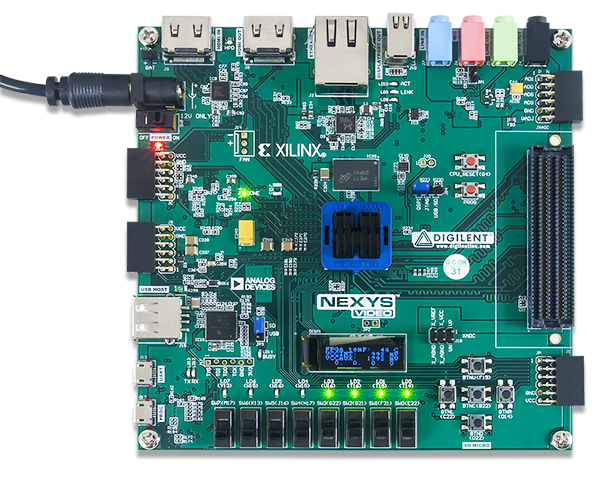
\includegraphics[width=0.7\linewidth]{nexys_video}
	\caption[Carte de développement Nexys Video]{Carte de développement Nexys Video. Source : digilent.com ref. URL02}
	\label{fig:nexys_video}
\end{figure}

\subsection{Encodage Cobs}

Une manière assez simple d’encoder un paquet et de le délimiter à l’aide de caractères spéciaux. 
C’est une méthode qui marche assez bien lorsque les données que l’on envoie sont limitées comme du texte par exemple. 
Toutefois, dans notre cas, nous souhaitons envoyer des données brutes qui peuvent contenir tout type de valeurs.

Il me fallait donc une méthode un peu plus poussée, c’est pour cela que je suis parti sur le \gls{cobs} qui est une méthode d’encodage assez légère et simple d’implémentation.

L’idée du \gls{cobs} est d’utiliser la valeur zéro comme indicatif de fin de paquet. 
Puis de remplacer tous les zéros présents dans le paquet d’origine par une valeur qui indique à combien d’octets, se trouve le prochain zéro. 
Un octet est ensuite ajouté au début du paquet pour indiquer la position du premier zéro dans les données originales. 
Ainsi, le paquet encodé ne contiendra qu’un seul zéro, situé à la fin, qui servira de marqueur pour indiquer la fin du paquet au destinataire. 
Au final, cette méthode est plutôt simple à mettre en place et rajoute seulement deux octets par rapport au paquet d’origine.

\begin{figure}[tbph!]
	\centering
	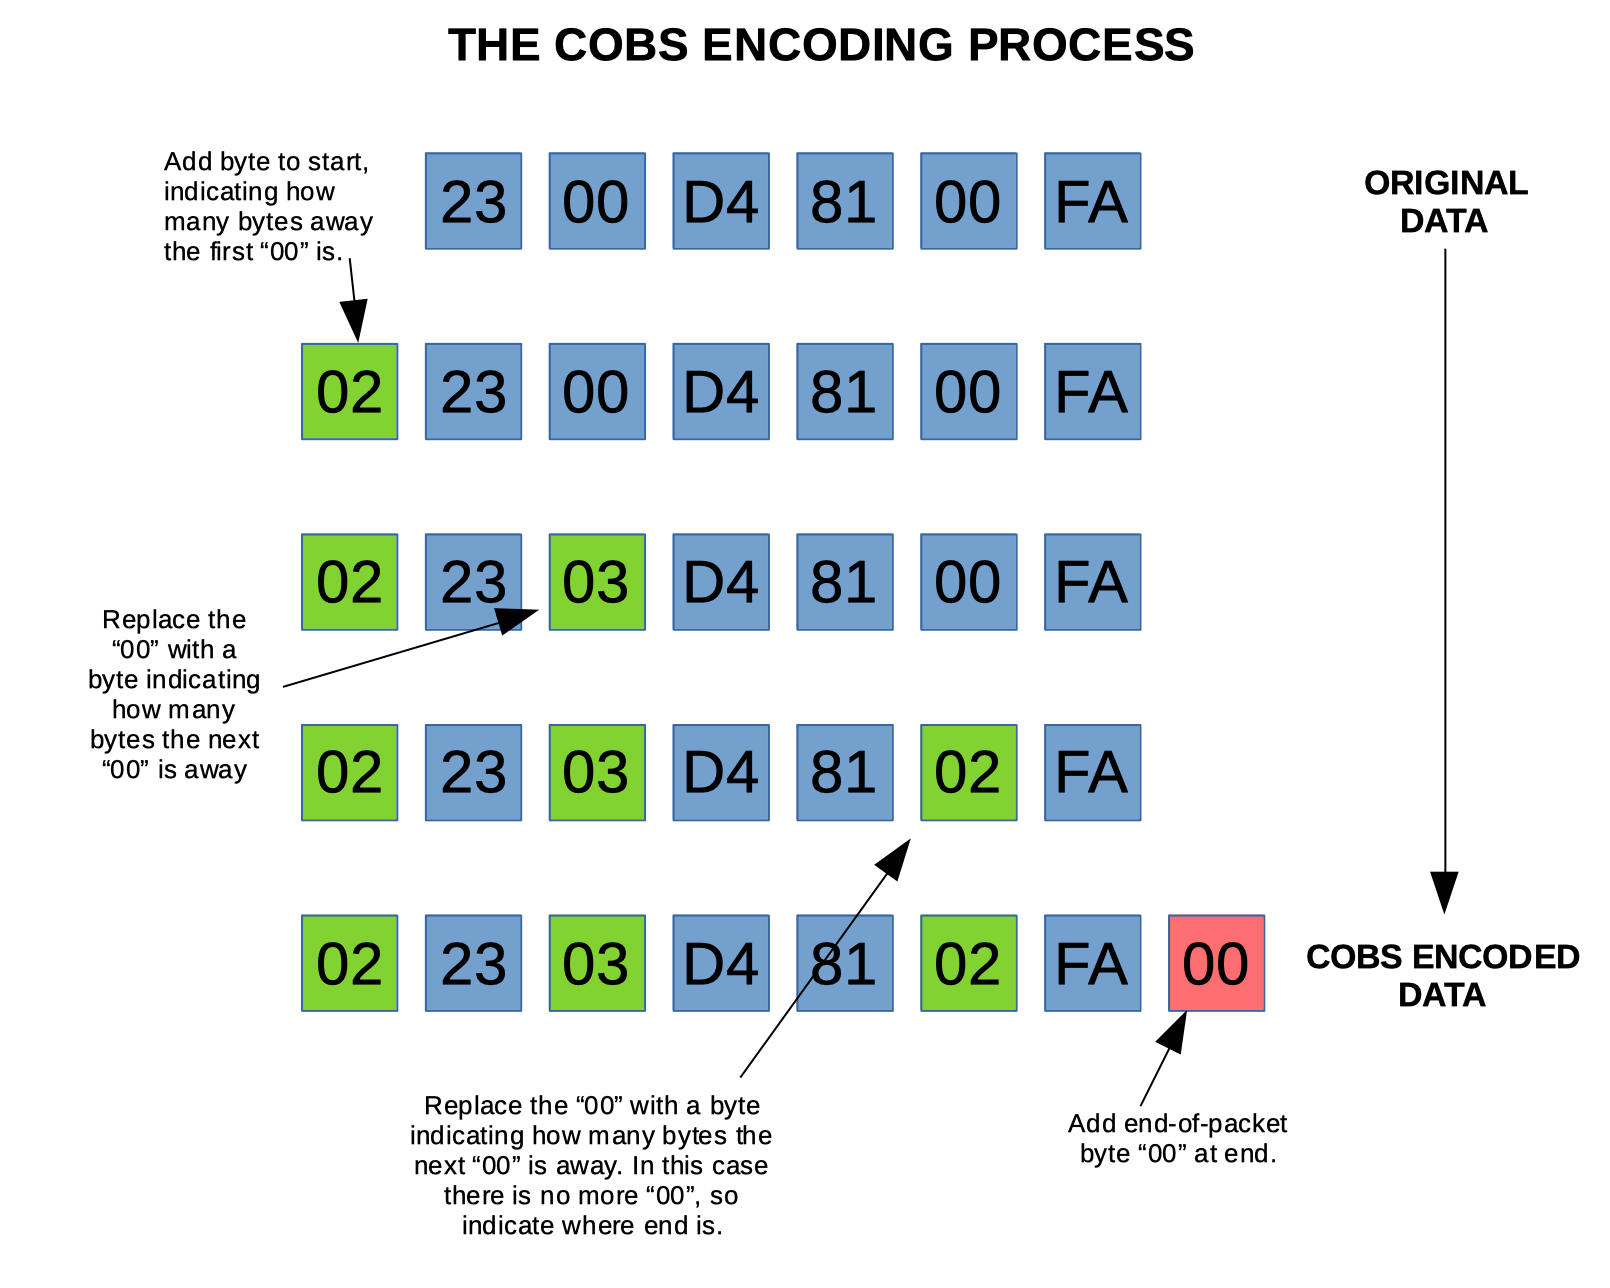
\includegraphics[width=0.7\linewidth]{cobs_encoding}
	\caption[Schéma Encodage COBS]{Schéma Encodage COBS. Source : blog.mbedded.ninja ref. URL03}
	\label{fig:cobs_encoding}
\end{figure}

\subsection{CRC}

Pour ce qui est de la vérification d'erreurs, l'algorithme utilisé de manière général est le \gls{crc}.
Après quelques recherches, je suis tombé sur un site internet\footcite{noauthor_generator_nodate} qui permet de générer du code dont du \gls{vhdl} en fonction du type de \gls{crc} souhaité.
Je suis parti sur le \gls{crc} le plus simple qui est le 8 bit, mais le code \gls{vhdl} nous est fourni sous forme de module, il est donc assez facile de remplacer le \gls{crc} par un autre plus rigide.

\subsection{Format et Type de Paquet}

Au final, tous les paquets doivent être structurer dans le même format en prenant compte de l'encodage et du \gls{crc}. 
J'ai aussi pris l'initiative pour être sûr d'ajouter un champ supplémentaire dans le paquet qui est la taille du paquet d'origine, car le paquet provenant de l'ordinateur devrait toujours être de la même taille. 

\begin{figure}[tbph!]
	\centering
	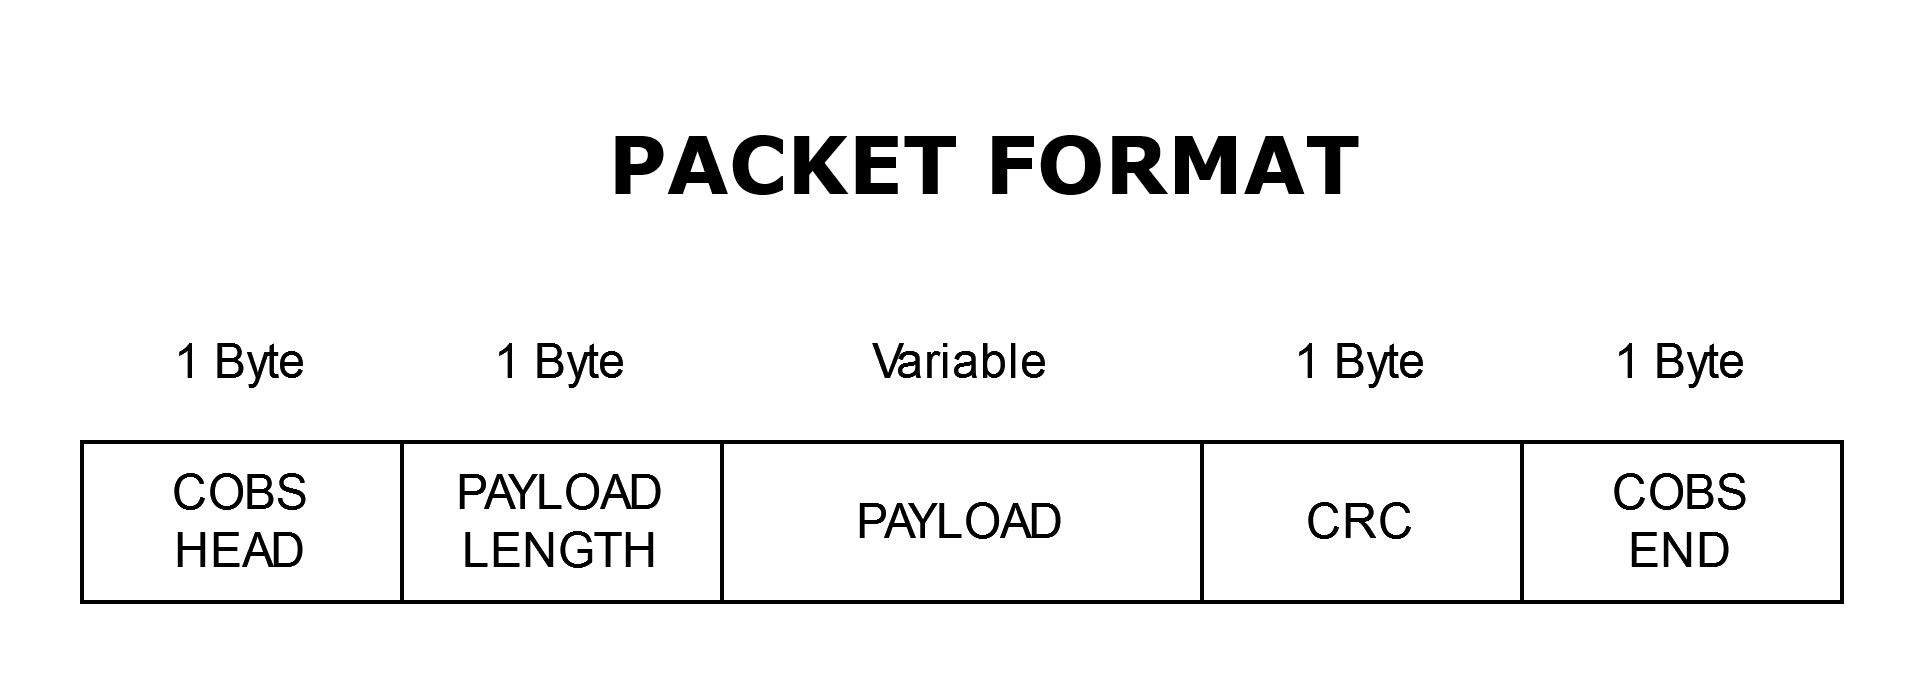
\includegraphics[width=0.6\linewidth]{uart_packet_format}
	\caption[Format de paquet - UART]{Format de paquet - UART. Source : réalisé par Kandiah Abivarman}
	\label{fig:uart_packet_format}
\end{figure}


\subsubsection{Paquet pour le FPGA}

Lorsque l'on souhaite faire une attaque, on doit envoyer un paquet pour configurer chaque quadcore.
De ce fait, on a qu'un seul type de paquet à envoyer et il faut en envoyer en fonction du nombre de quadcore présent dans le \gls{fpga}.

\begin{figure}[tbph!]
	\centering
	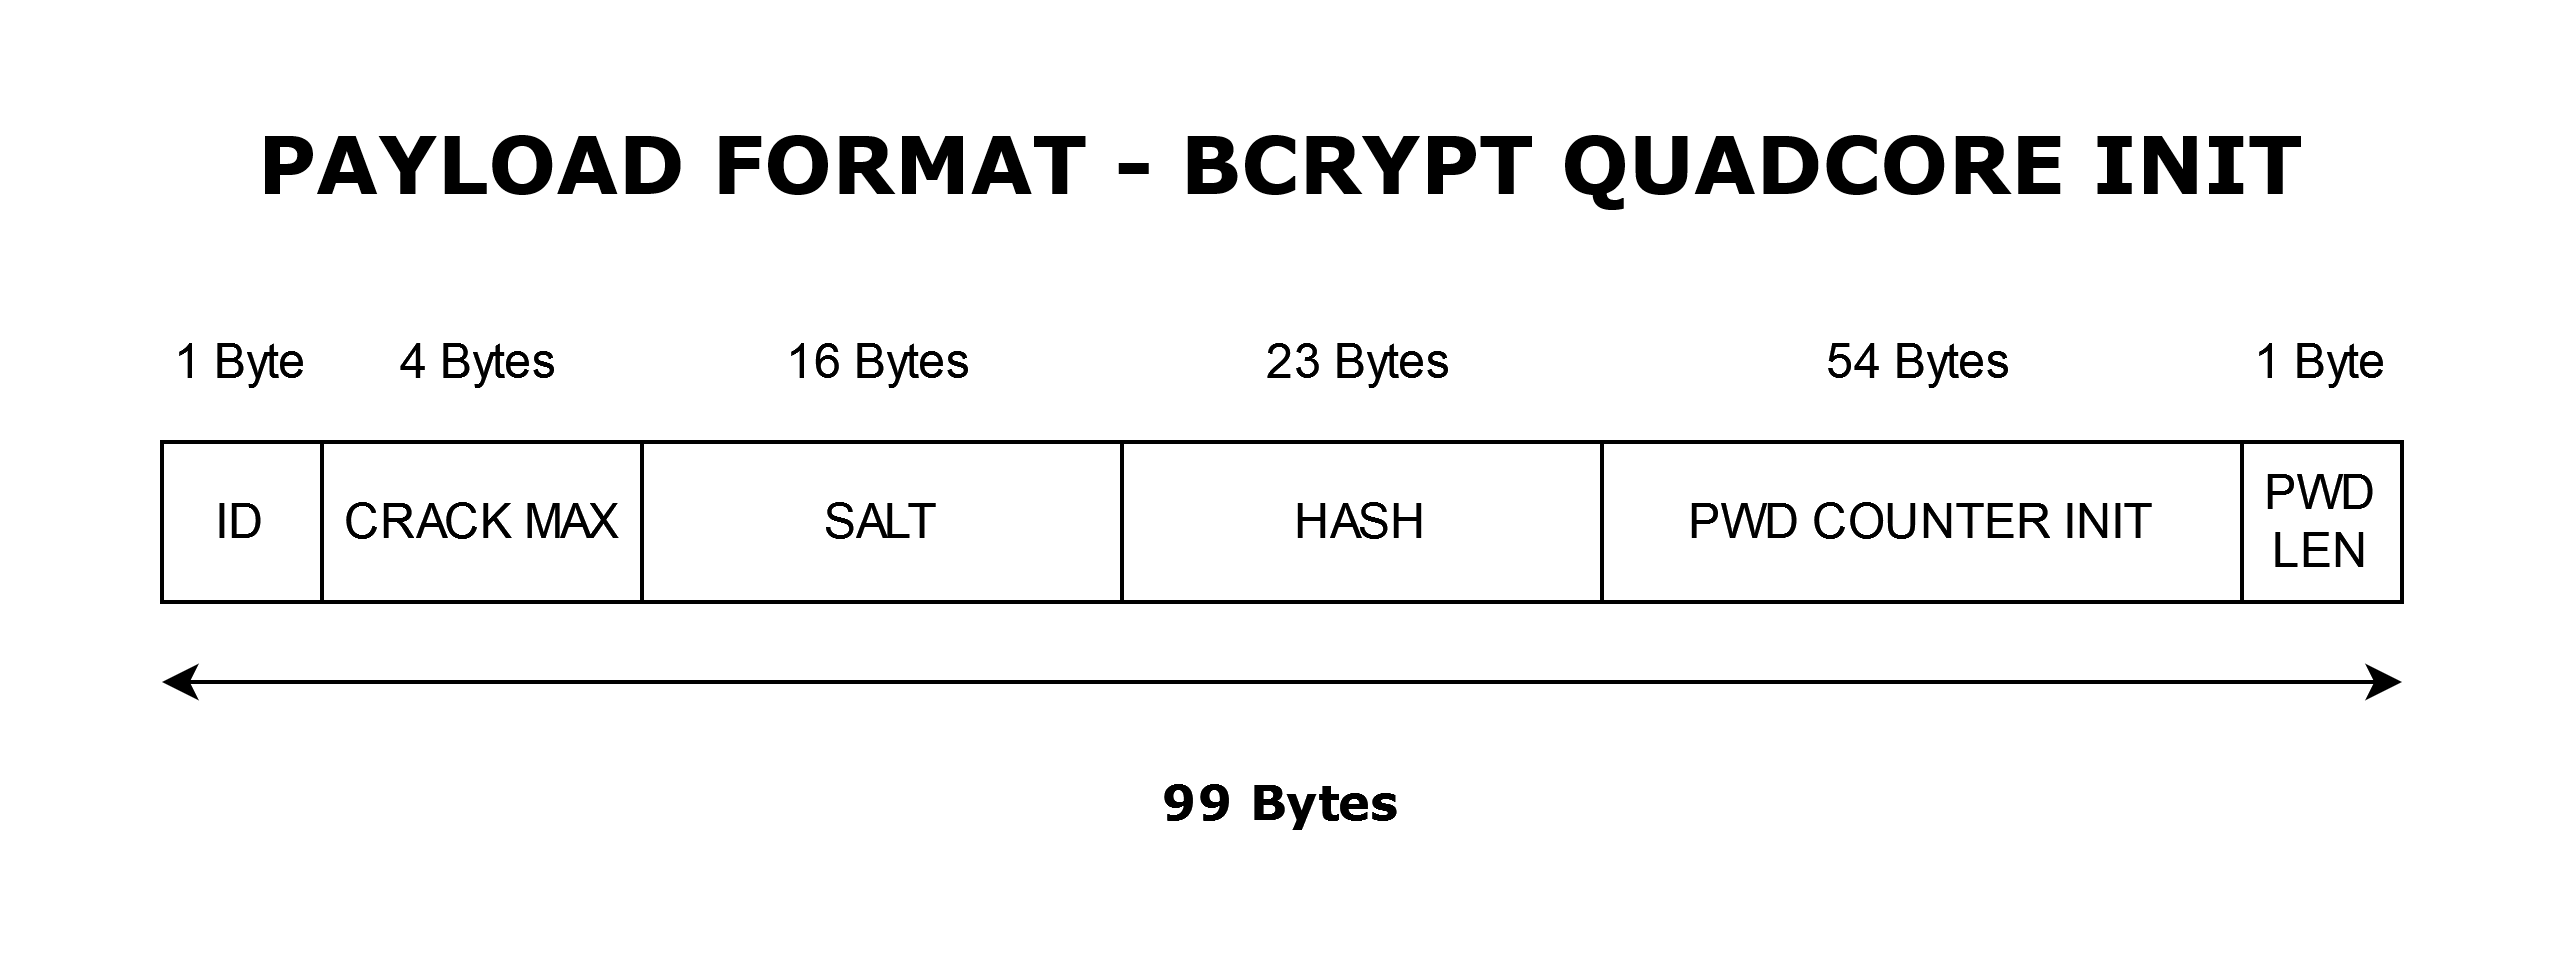
\includegraphics[width=0.7\linewidth]{uart_mosi_payload_format}
	\caption[Format de paquet - MOSI]{Format de paquet - MOSI. Source : réalisé par Kandiah Abivarman}
	\label{fig:uart_mosi_payload_format}
\end{figure}

\newpage

\subsubsection{Paquet pour l'ordinateur}

Lorsque le \gls{fpga} recevra un paquet, il devrait envoyer un paquet de réponse afin d'avertir l'ordinateur de la bonne réception du paquet.

\begin{figure}[tbph!]
	\centering
	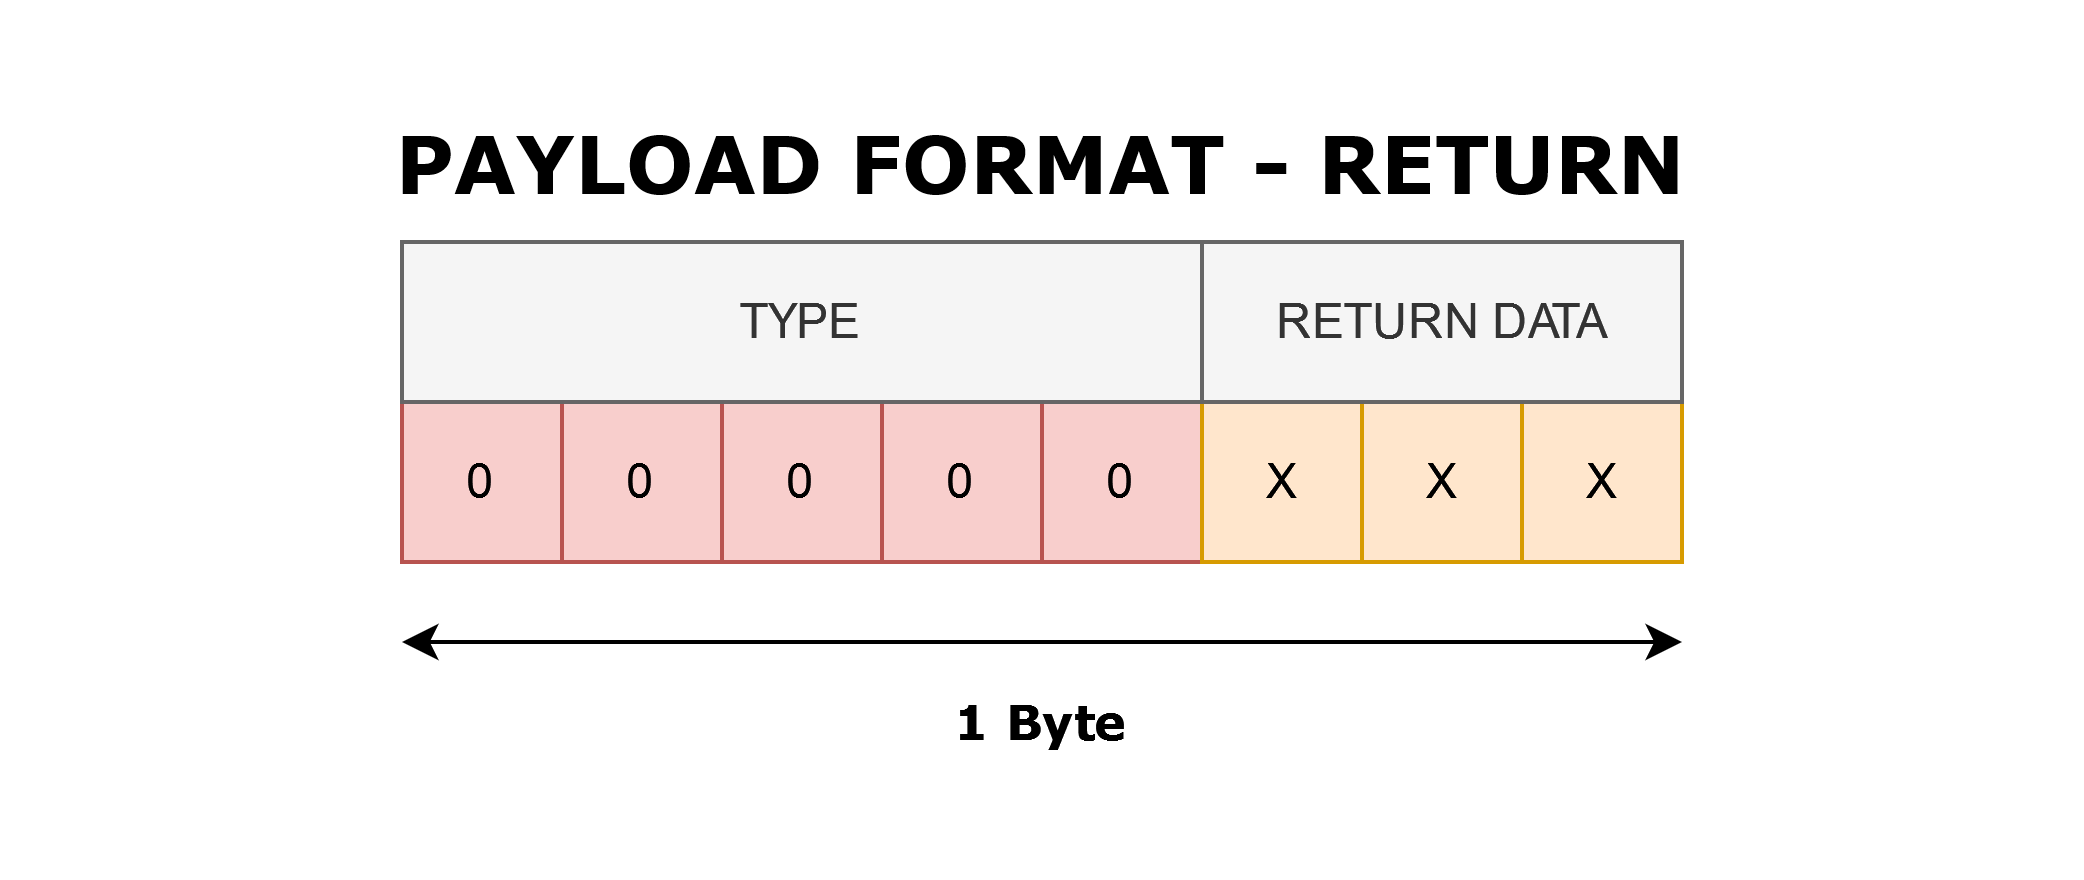
\includegraphics[width=0.7\linewidth]{uart_return_payload_format}
	\caption[Format de paquet - Retour]{Format de paquet - Retour. Source : réalisé par Kandiah Abivarman}
	\label{fig:uart_return_payload_format}
\end{figure}

Lorsque le paquet est une réponse, le champ type vaudra zéro est les trois bits de point faibles vont nous indiquer l'erreur si il y en a une.\\

\begin{table}[tbph!]
	\centering
	\begin{tabular}{|c|c|}
	\hline
	\textbf{Return Code} & \textbf{Return}                   \\ \hline
	000                  & OK                                \\ \hline
	001                  & Packet size greater than expected \\ \hline
	010                  & Packet size smaller than expected \\ \hline
	011                  & Quadcore ID not valid             \\ \hline
	100                  & CRC Error                         \\ \hline
	\end{tabular}
	\caption{Tableau de code d'erreur - Paquet UART}
	\label{tab:error_code_uart}
\end{table}

Quand le paquet n'est pas une réponse alors les trois bits vaudront zéros et pourront être ignoré. 

\newpage

En dehors d'une réponse, le \gls{fpga} envoyera aussi un paquet toutes les secondes pour donner l'état d'avancement de l'attaque.
Puis, bien évidemment un paquet sera aussi envoyer lorsque le mot de passe cherché sera trouvé.

\begin{figure}[tbph!]
	\centering
	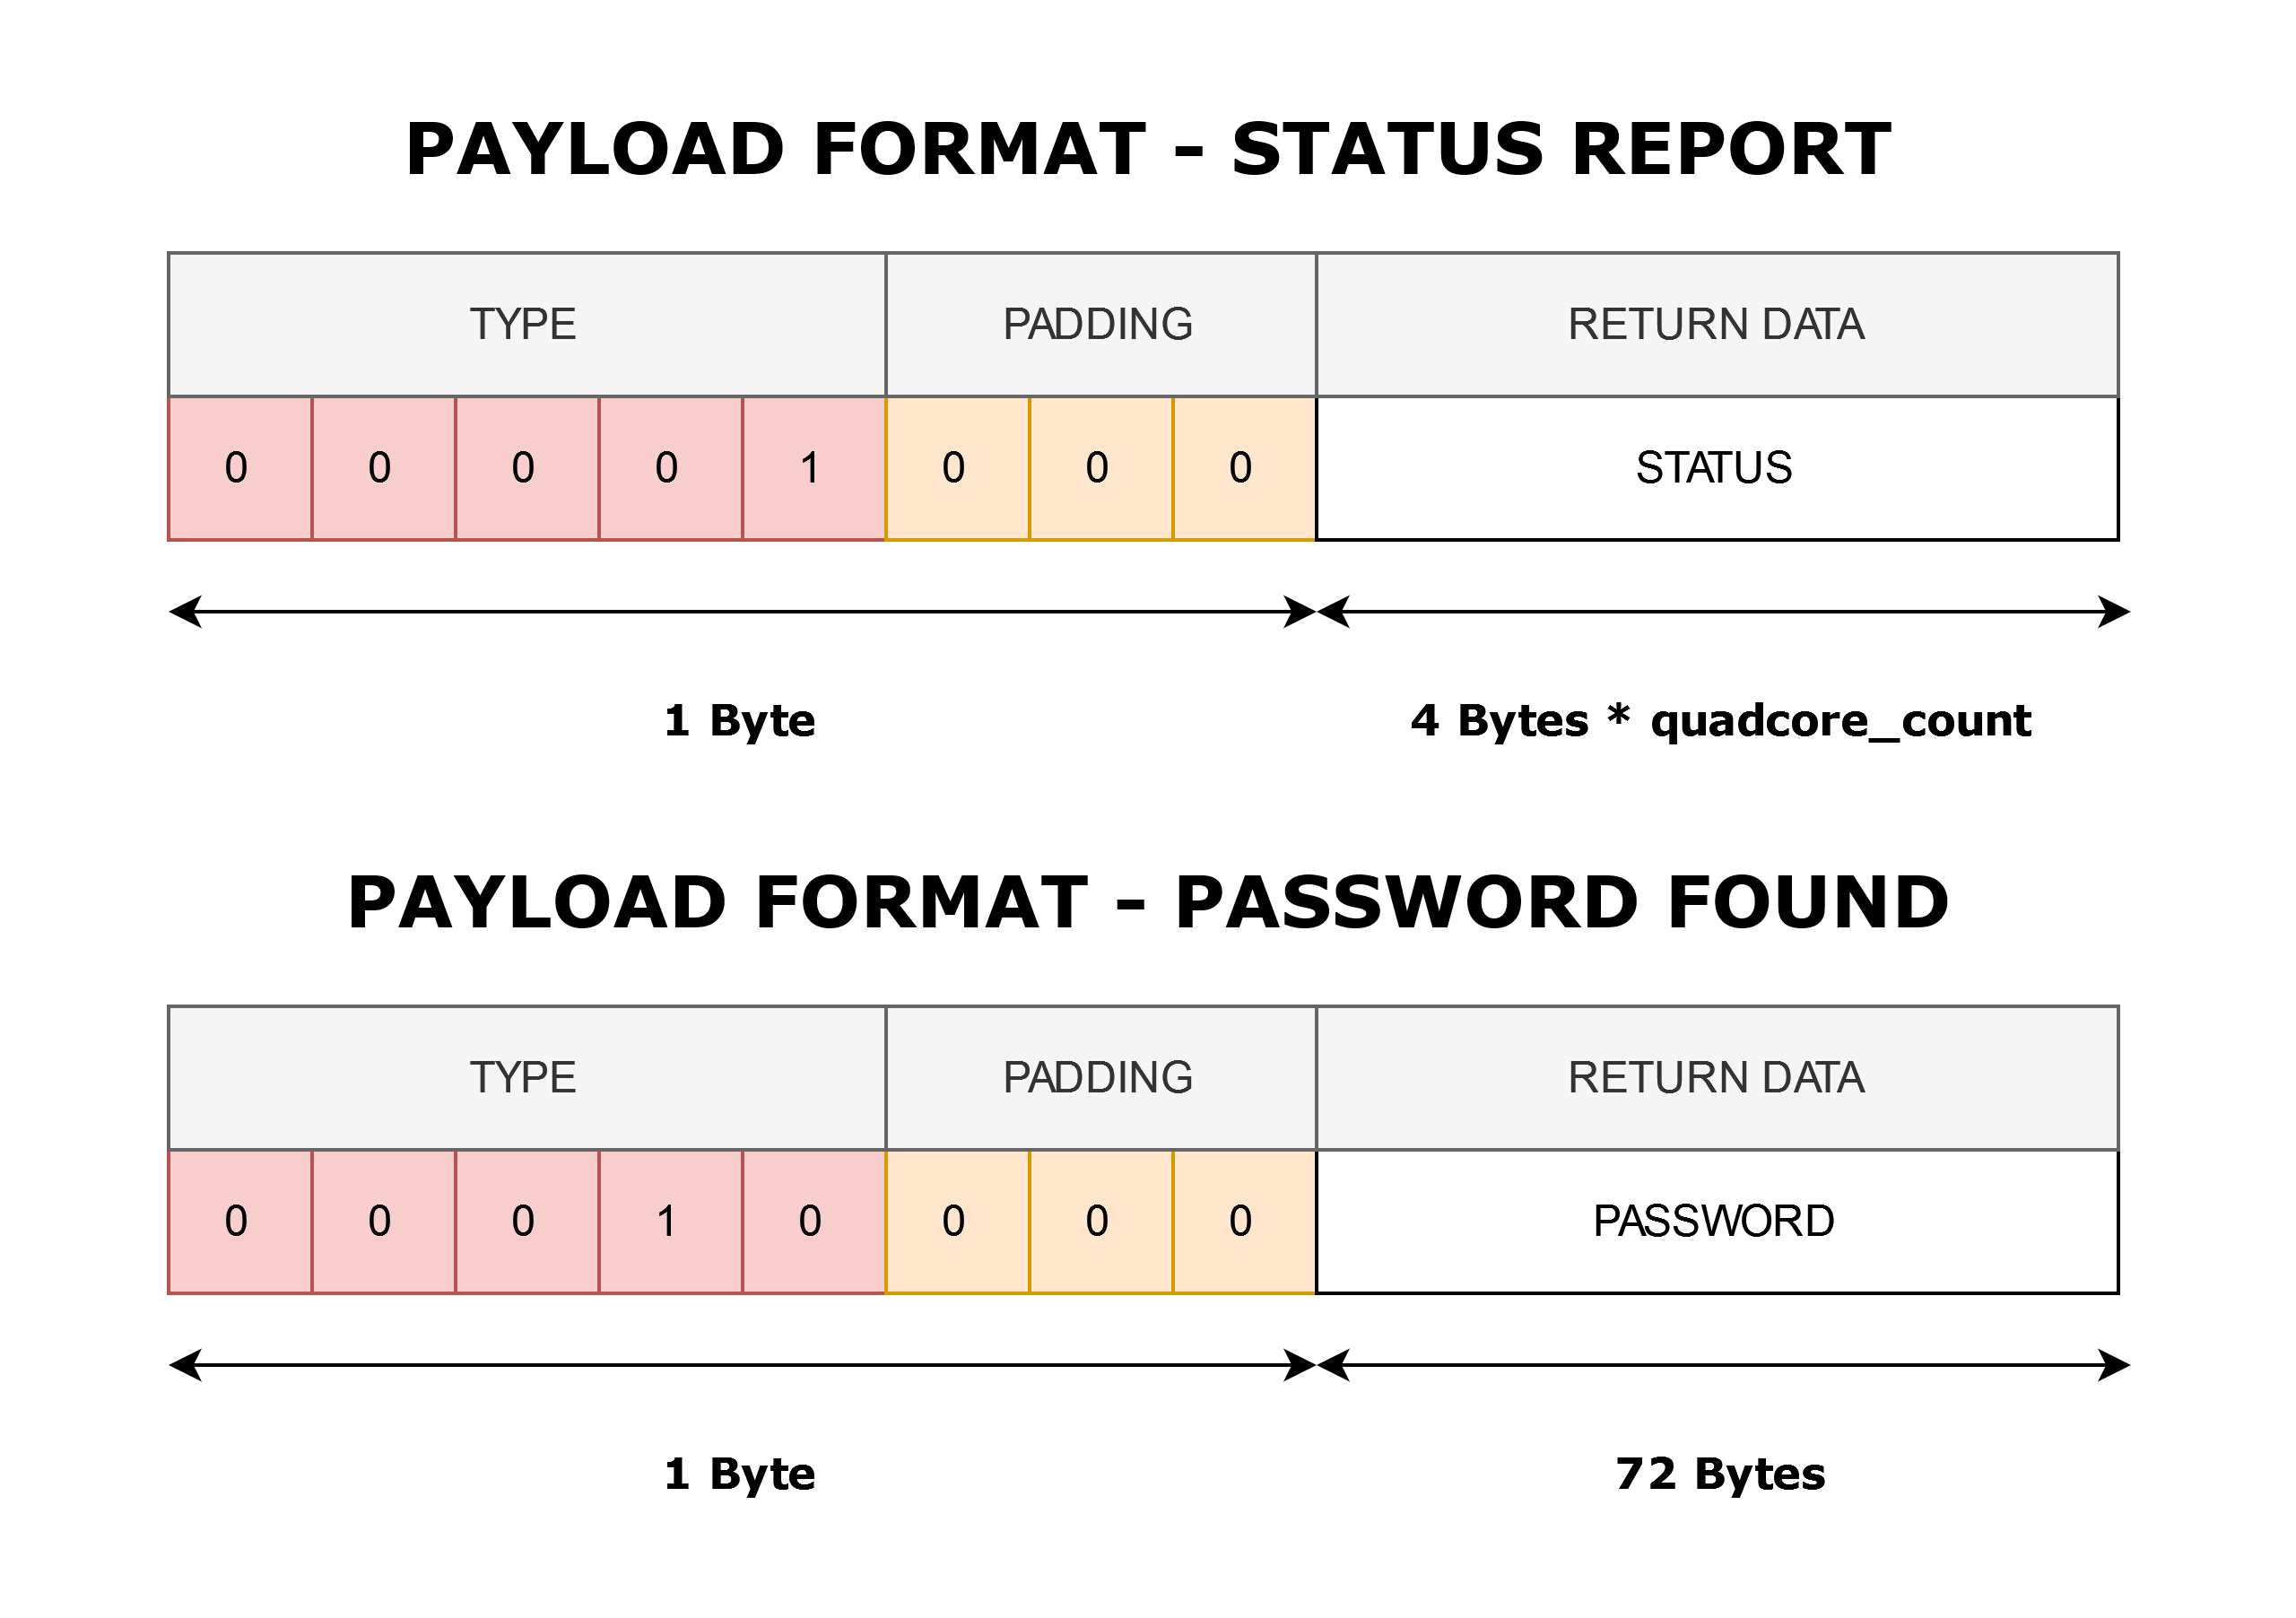
\includegraphics[width=0.7\linewidth]{uart_miso_payload_format}
	\caption[Format de paquet - MISO]{Format de paquet - MISO. Source : réalisé par Kandiah Abivarman}
	\label{fig:uart_miso_payload_format}
\end{figure}

\newpage

\section{Implémentation Solution UART}

\subsection{Architecture Logique}

Pour la partie implémentation, j’avais déjà un module \gls{uart} en \gls{vhdl} qui marchait et le bcrypt cracker fonctionnel lorsque réglage était codé en dur. 
Il fallait donc que je mette en place tout ce qui allait avoir entre l’interface \gls{uart} et le système d’attaque bcrypt, c’est-à-dire toute la partie gestion de paquet. 
J’ai aussi dû adapter le module bcrypt cracker et quadcore afin qu’il puisse marcher correctement avec l’architecture souhaitée.

Pour le module qui allait s’occuper des paquets, j’ai pensé à diviser cette partie en deux. 
Une première partie qui allait s’occuper de la réception des paquets, donc le décodage, la vérification et ressortir les données pour les quadcores. 
Puis une deuxième partie qui doit gérer toute la partie transmission des paquets de retours, de statut et du mot de passe trouvé. 
Les deux modules seront reliés de ce fait, lorsque il y aura un souci ou non avec un paquet reçu, le module de réception pourra avertir le module de transmission afin qu’il puisse envoyer le paquet de retours.

\begin{figure}[tbph!]
	\centering
	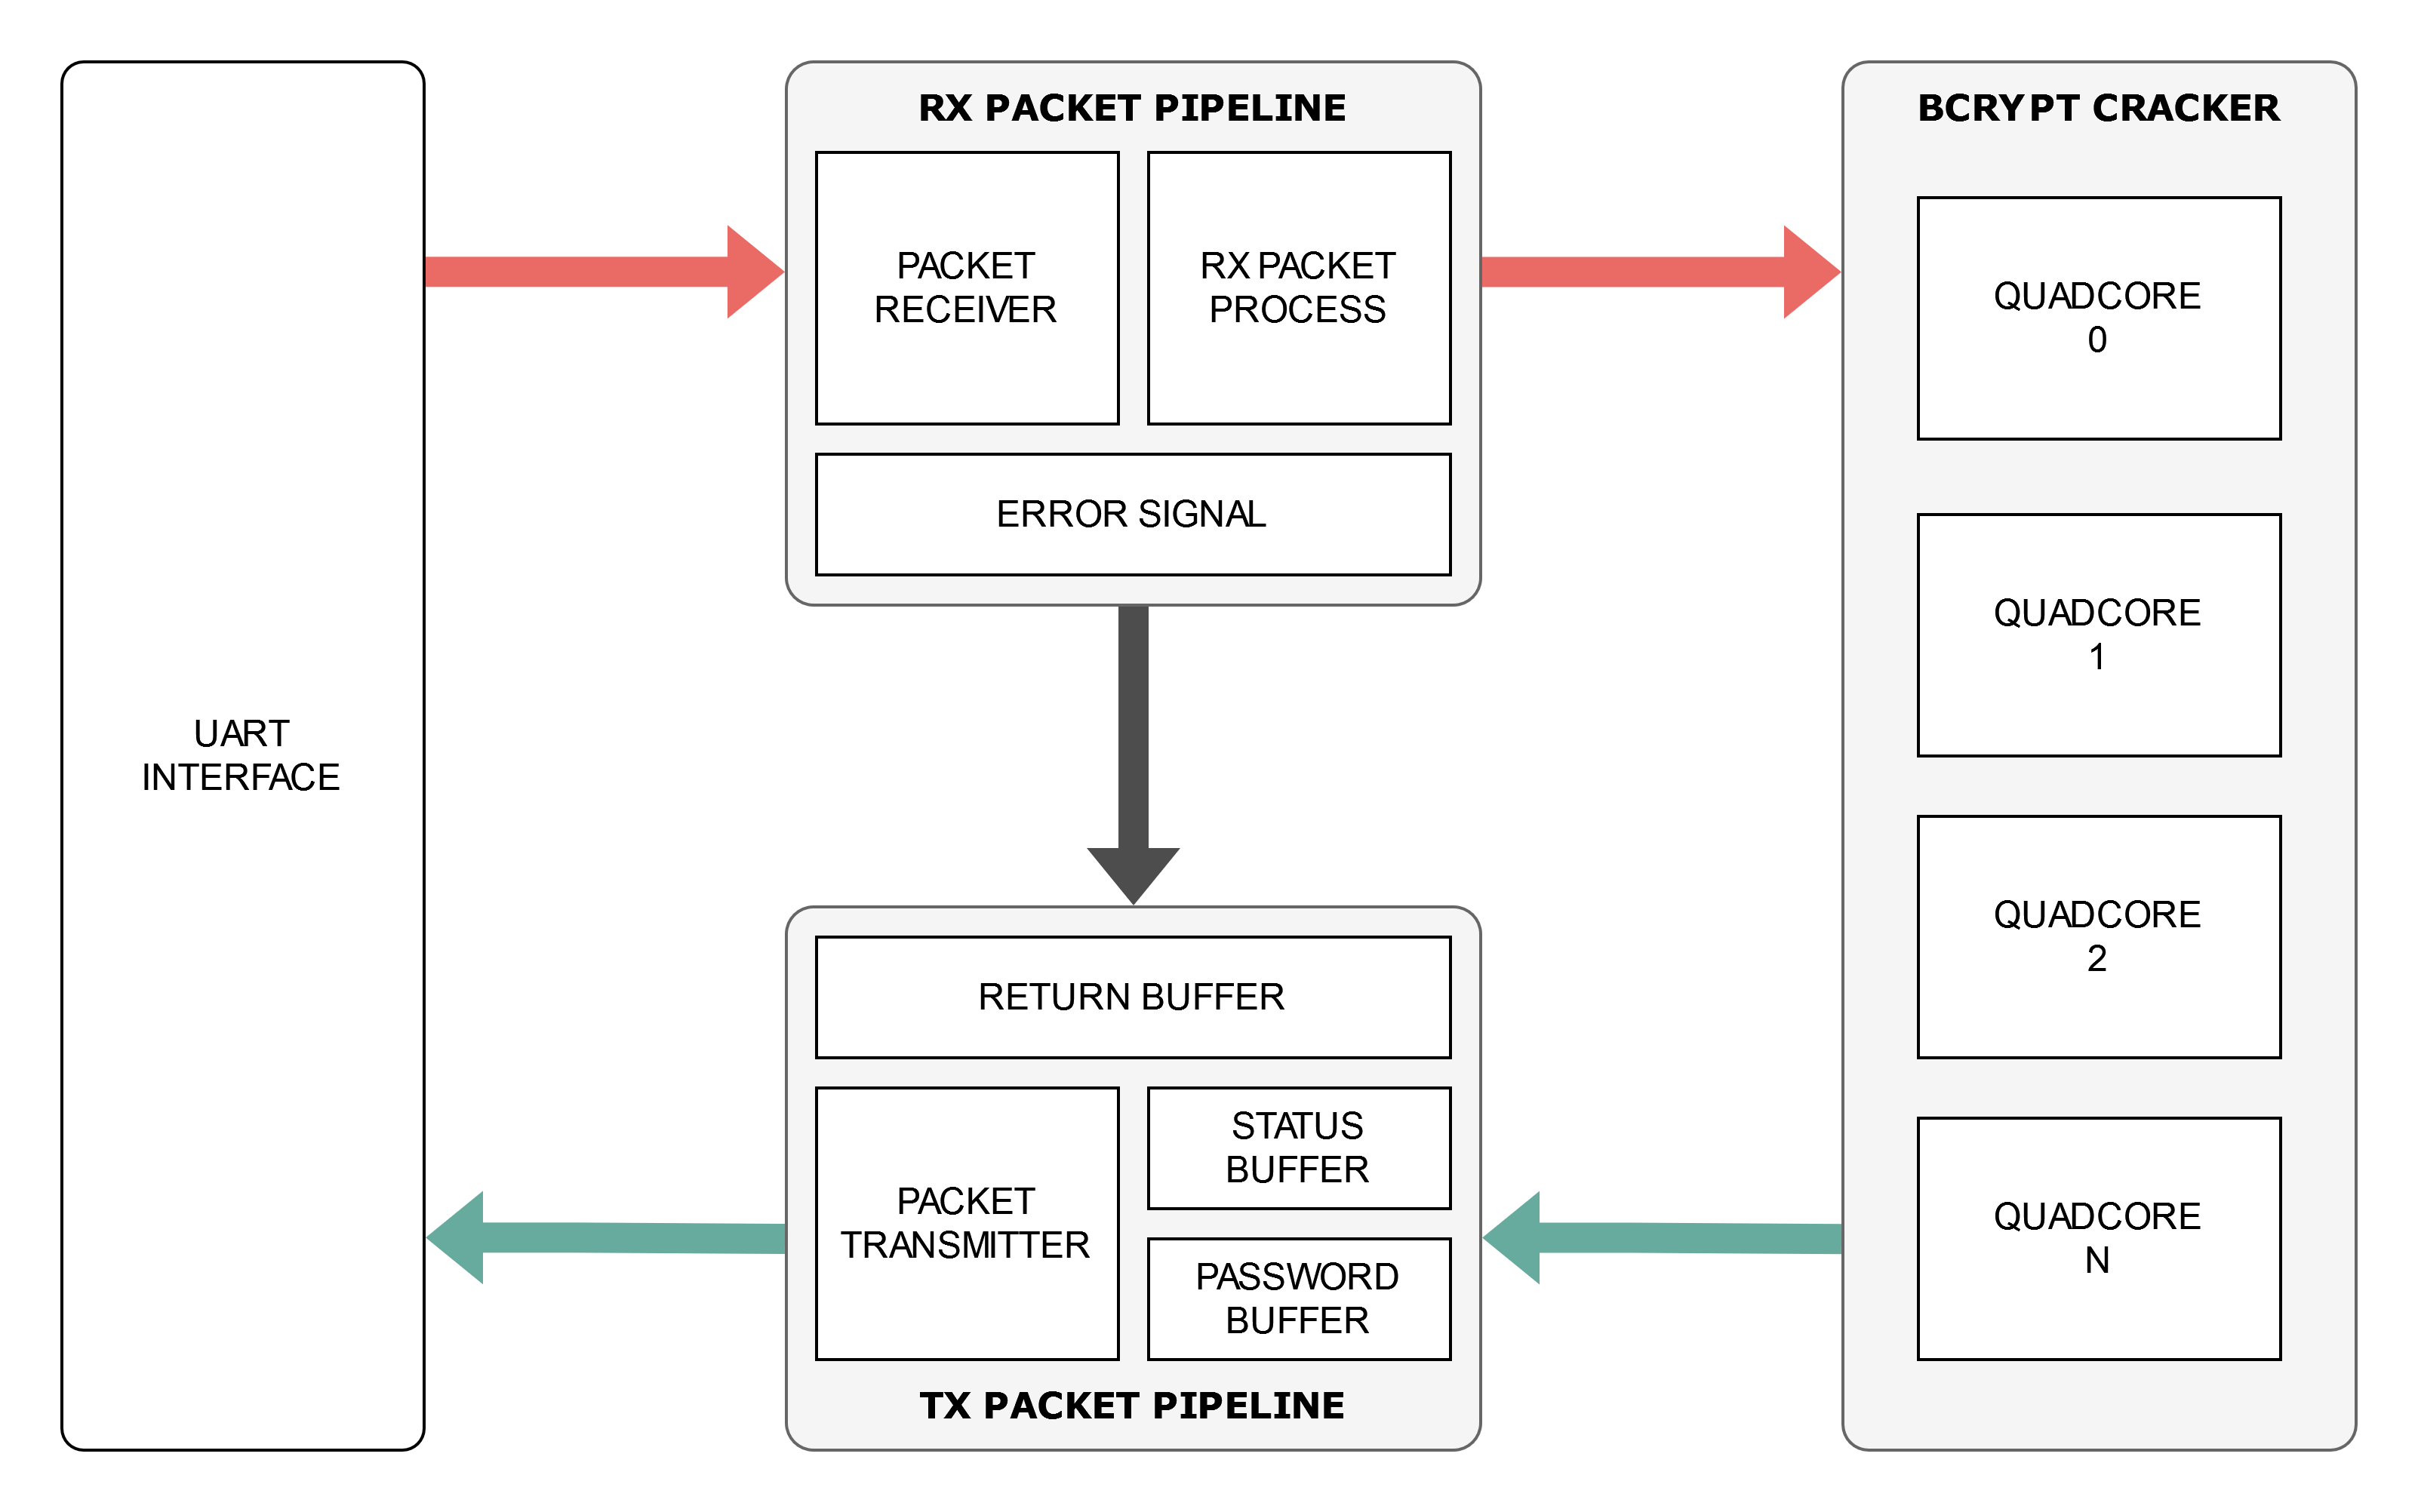
\includegraphics[width=0.7\linewidth]{uart_communication_protocol_top_rev2}
	\caption[Schéma système UART - FPGA]{Schéma système UART. Source : réalisé par Kandiah Abivarman}
	\label{fig:uart_top_schematics}
\end{figure}


\subsection{Implémentation - MOSI}

La gestion de la réception de paquet va être composée tout d’abord d’un module Packet Receiver qui va s’occuper de décoder et de calculer le \gls{crc} et vérifier le \gls{crc} du paquet reçu. 
Ensuite, il y a le RX Packet Process qui va s’occuper de récupérer les données qui ont été décodées et de ressortir les données dans le bon format pour le bcrypt cracker. 
Pour finir, il y a le RX Packet Pipeline qui va s’occuper d’instancier les deux modules et de récupérer les erreurs provenant de ceux-ci.

\subsubsection{Module - Packet Receiver}

Ce module s'occupe de récupérer byte par byte les données reçus par \gls{uart}, puis de les décoder immédiatement afin de les exposer en sortie.
Suite au décodage, le \gls{crc} sera calculé afin qu'il puisse être comparé avec le \gls{crc} réceptionné à la fin du paquet.
Après vérification du \gls{crc}, une sortie sera mis à un, afin de signaler le module qui va récupérer les données que ceux-ci sont bien valides.

\begin{figure}[tbph!]
	\centering
	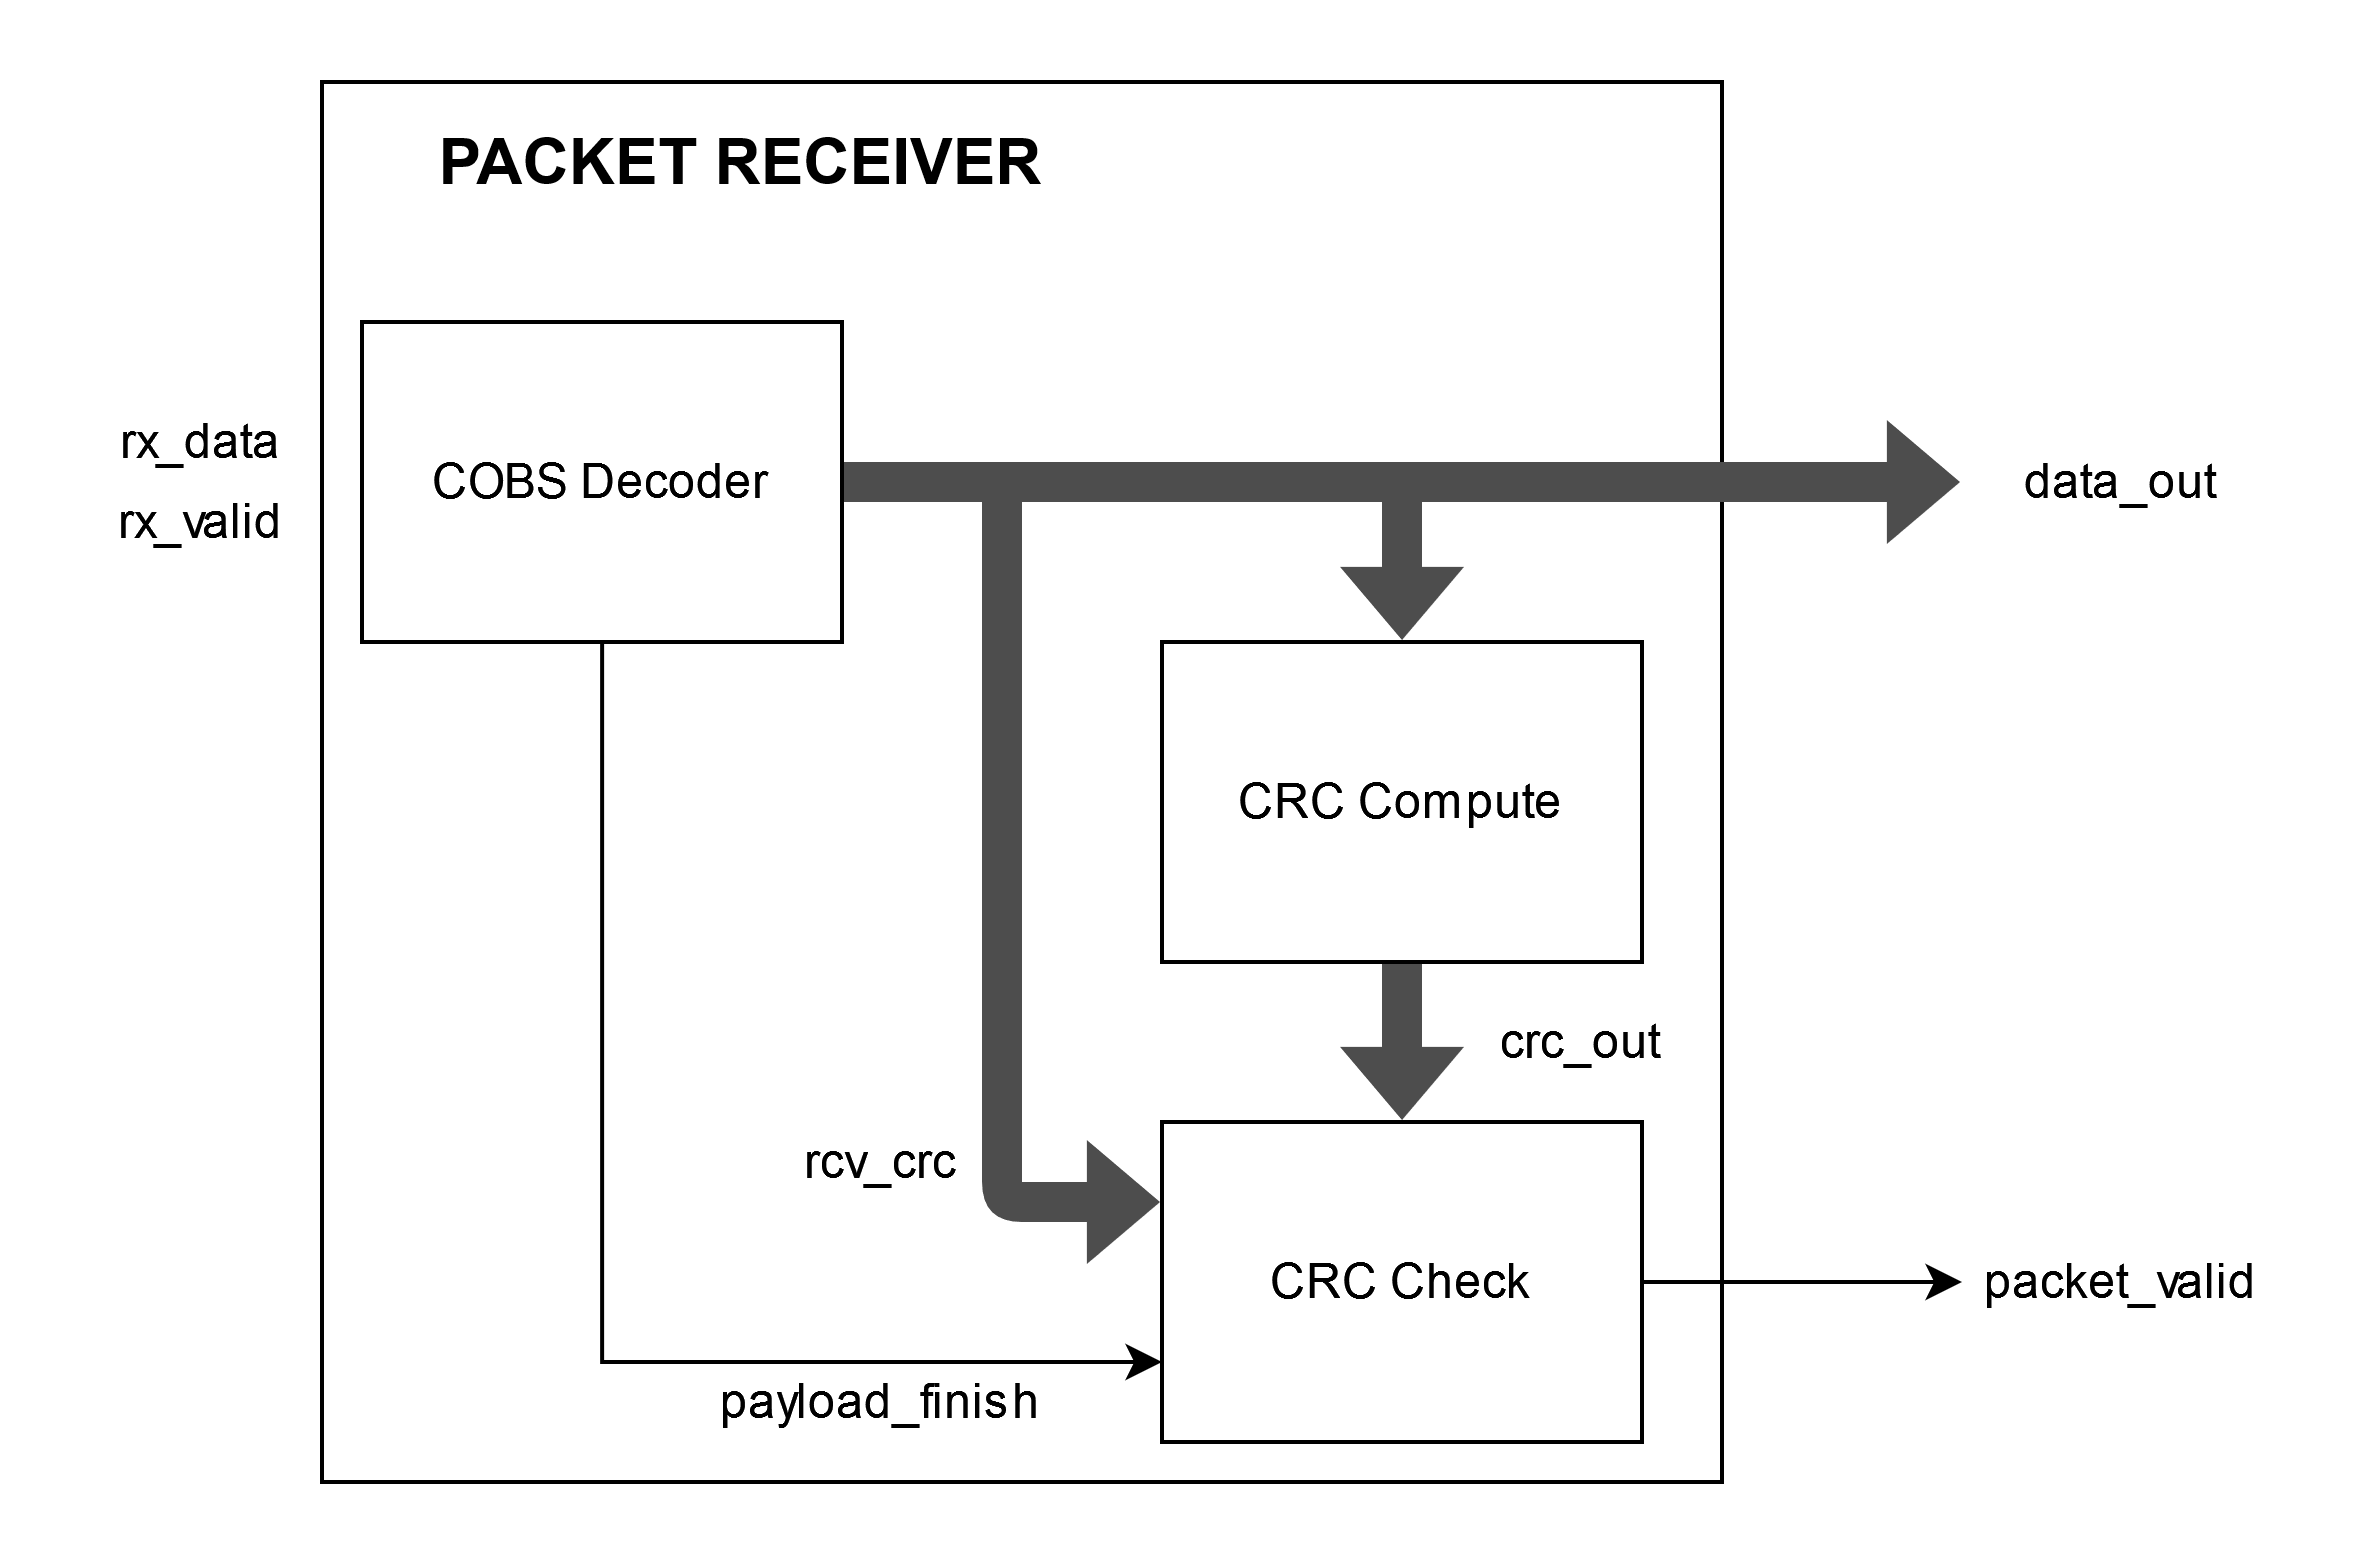
\includegraphics[width=0.7\linewidth]{uart_packet_receiver}
	\caption[Schéma Packet Receiver]{Schéma Packet Receiver. Source : réalisé par Kandiah Abivarman}
	\label{fig:uart_packet_receiver}
\end{figure}


\subsubsection{Module - RX Packet Process}

Ce module va récupérer les données décodées du Packet Receiver et les stockés.
Lorsque le module a réceptionné le paquet entier, il va vérifier à l'aide d'un signal émis par le module précèdent si le paquet est valide.
Si le paquet n'est pas valide, alors les données reçues seront ignorés et le module attendra un nouveau paquet.
Toutefois si le paquet est bien valide, d'autres facteurs vont être vérifié, tels que la taille du paquet ou encore l'adressage du quadcore.
En effet, si le paquet ne fait pas la taille attendu ou encore le quadcore ciblé n'est pas valide, alors le module va lui aussi signaler dans une sortie le type d'erreur.
Au final, si tout est bon alors, le module va ressortir les données dans le bon format pour le bcrypt cracker et le bcrypt quadcore.

\begin{figure}[tbph!]
	\centering
	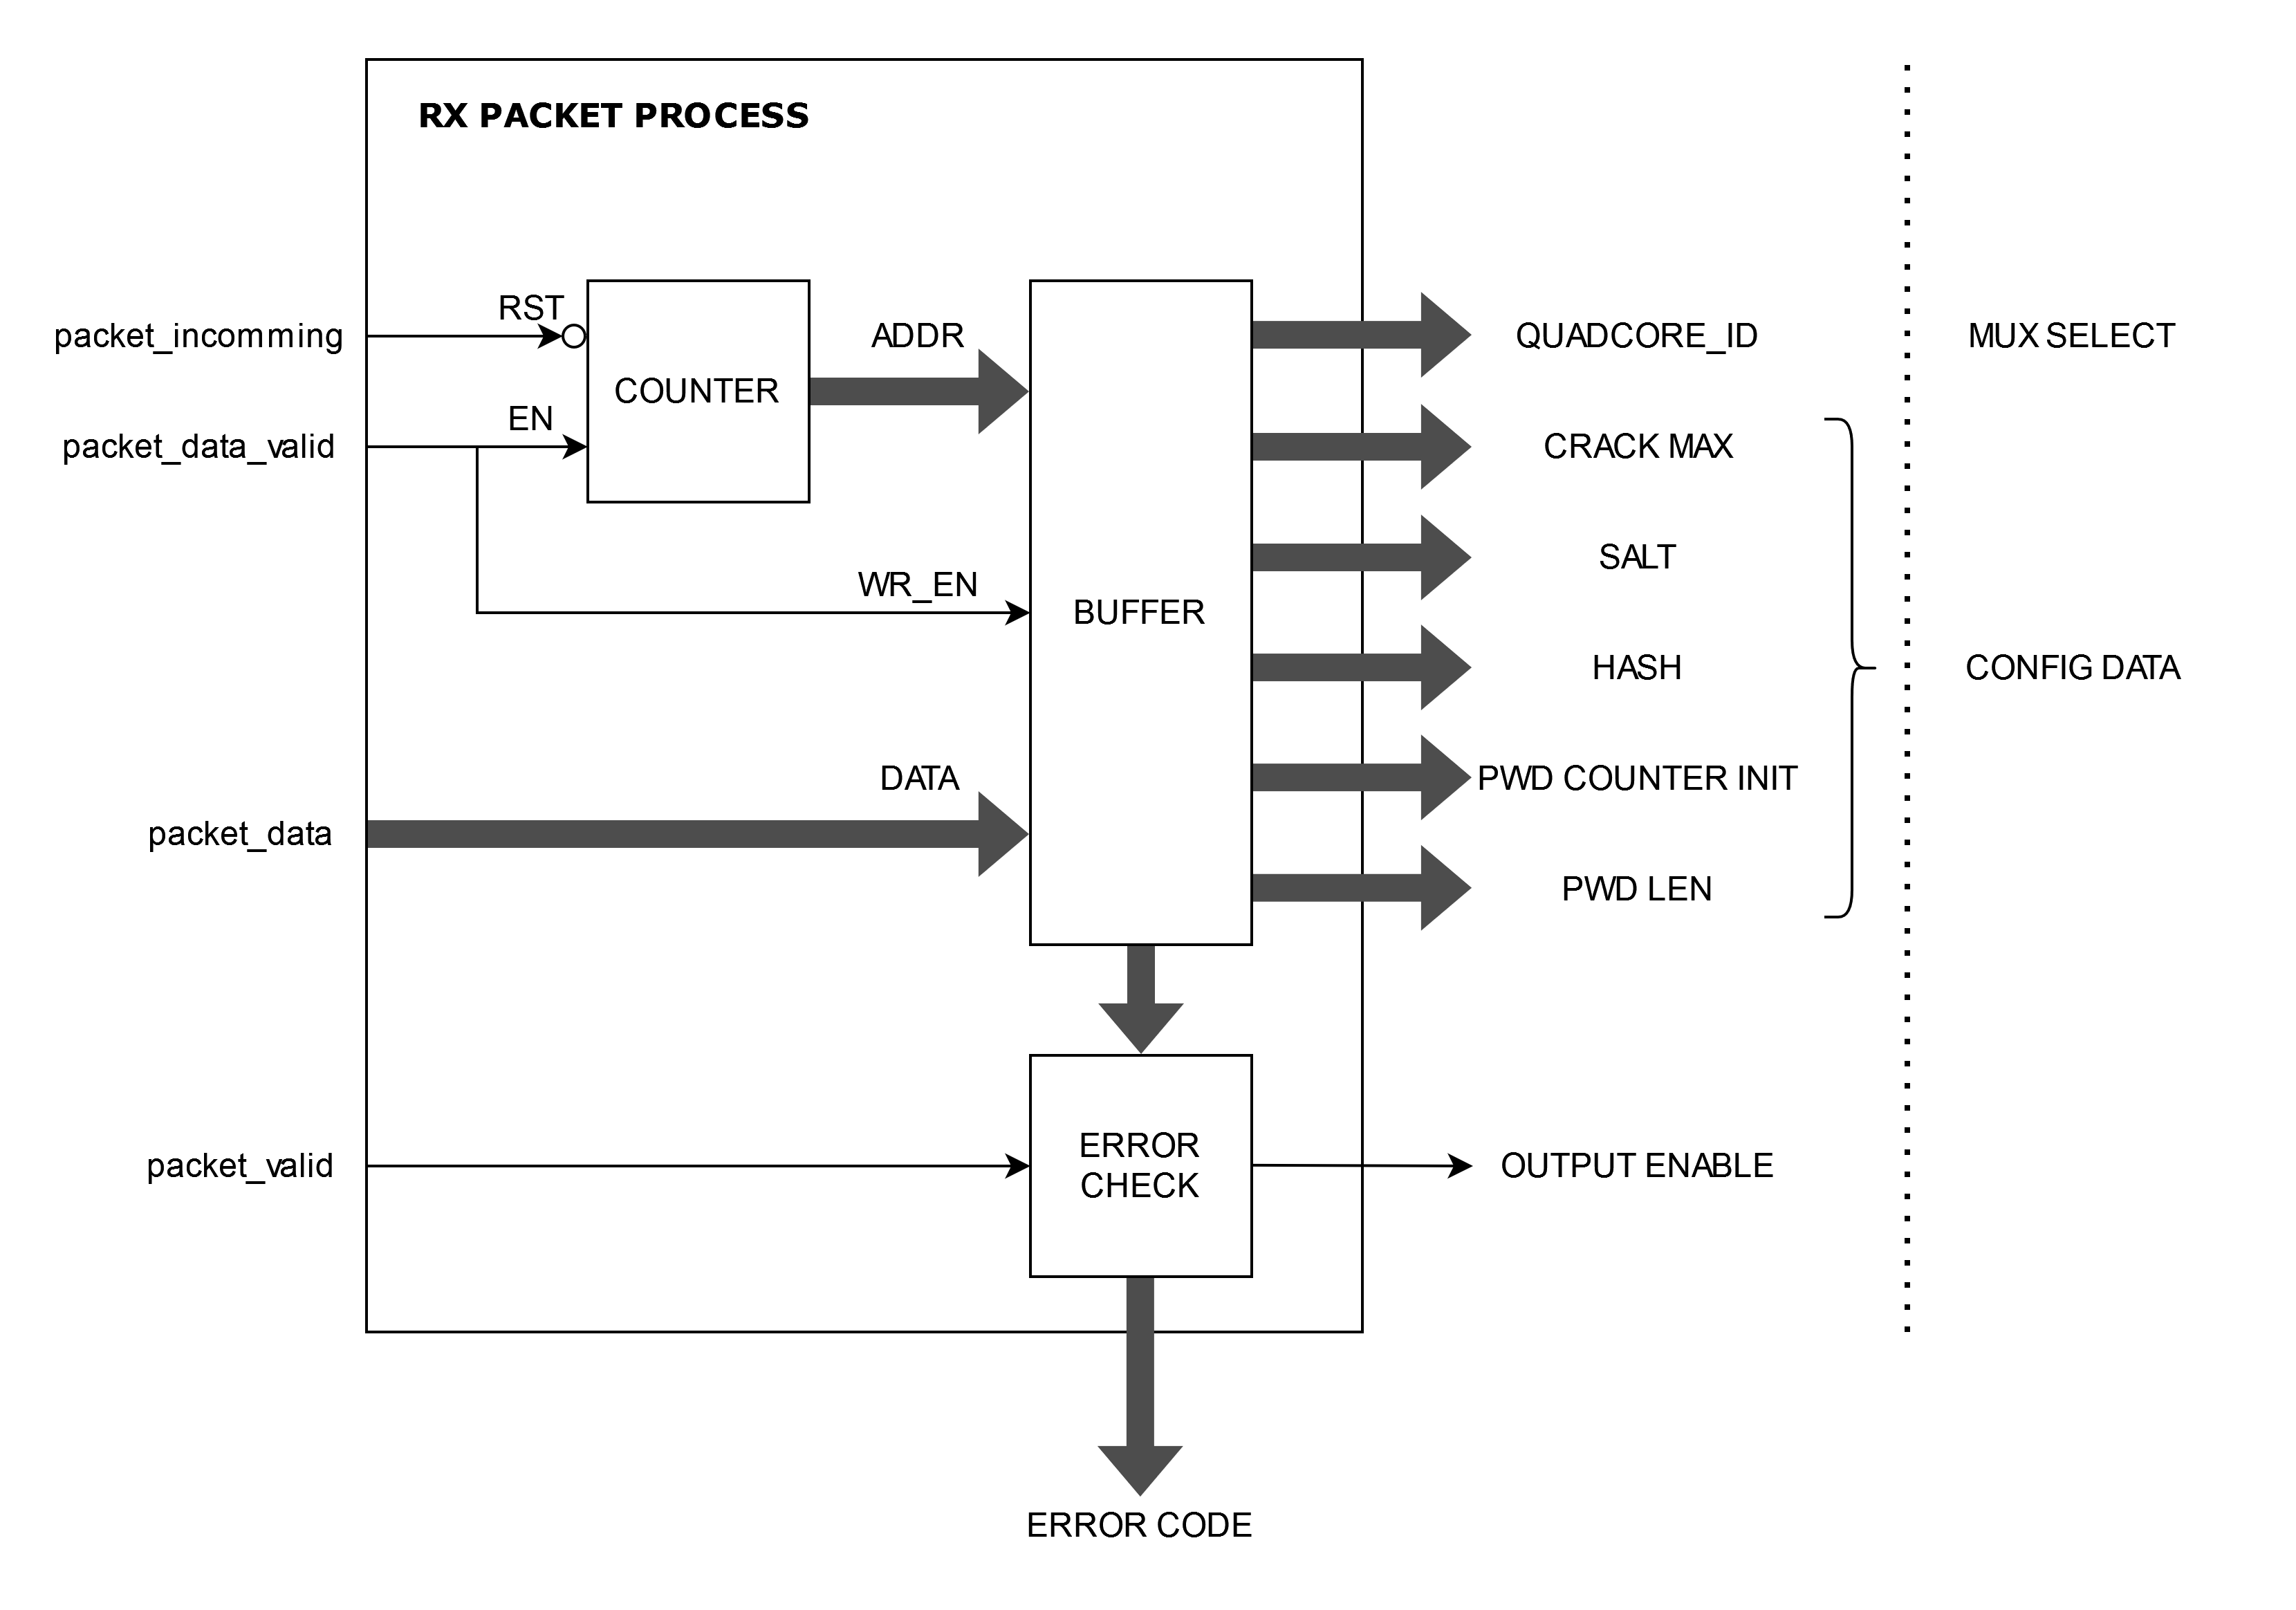
\includegraphics[width=0.7\linewidth]{uart_rx_packet_process}
	\caption[Schéma RX Packet Process]{Schéma RX Packet Process. Source : réalisé par Kandiah Abivarman}
	\label{fig:uart_rx_packet_process}
\end{figure}

\subsubsection{Module - RX Packet Pipeline}

Le RX Packet Pipeline est un module qui sert principalement à instancier les deux modules précédemment vus.
Le module va aussi s'occuper de recupérer les signaux d'erreurs provenant des deux autres modules et les exposer afin qu'elles puissent être utilisé pour le paquet de retour.   

\subsection{Implémentation - MISO}

La gestion de la transmission des paquets va être scindée en deux modules.
On a tout d'abord le TX Packet Pipeline qui est le module qui va décider quel type de paquets va être envoyé.
Puis il y a le Packet Transmitter qui à l'inverse du Packet Receiver va s'occuper d'ajouter un \gls{crc} et d'encoder le paquet afin qu'il puisse être envoyé par \gls{uart}. 
Le Packet Transmitter est instancié à l'intérieur du TX Packet Pipeline.

Cette partie du travail, a été celui avec lequel j'ai eu le plus de difficultés dans le système au complet.

\newpage

\subsubsection{Module - TX Packet Pipeline}

Ce module va permettre de former les différents type de paquets qui seront envoyés à l’ordinateur.

La logique du module peut être séparée en quatre processus bien distincts :
\begin{enumerate}
	\item On a un processus qui s’occupe de récupérer le retour du RX Packet Pipeline afin de mettre en place un paquet de retours.
	\item L’autre processus va s’occuper de récupérer chaque seconde le nombre d’attaques effectué par chaque quadcore pour en faire un paquet.
	\item Ce processus, qui est le plus important, va attendre que le mot de passe soit trouvé puis récupérer le mot de passe afin d’en faire un paquet.
	\item Le dernier processus est là pour sélectionner quel paquet va être envoyé, lorsque un ou plusieurs processus sont prêts à envoyer leur paquet.
\end{enumerate}

J’ai aussi mis en place un système de priorité, entre les différents type de paquet. 
Le paquet de réussite a donc la plus grande priorité, suivi du paquet de retours puis pour finir le paquet de statuts.

\subsubsection{Module - Packet Transmitter}

Lorsque le paquet est prêt à être envoyé, ce module va récupérer octet par octet le paquet et le stocker.
Durant le stockage du paquet, le \gls{crc} sera calculé en même temps.

Suite au stockage de l'intégralité du paquet, le \gls{crc} calculé y sera ajouté et l'encodage \gls{cobs} sera effectué.

Puis lorsque le paquet sera entièrement traité, il sera envoyé à l'interface \gls{uart}.

\subsection{Modifications Bcrypt Cracker}

Afin que le bcrypt cracker puisse s'interfacer correctement avec le système de paquets, j'ai dû le modifier lui et le bcrypt quadcore.

À la base, l'état initial du générateur de mots de passe et le nombre d'attaques limite étaient tout deux écrit à la dure dans le code pour chaque quadcore.
De ce fait, au démarrage tous les quadcores démarraient immédiatement l'attaque en même temps.

J'ai donc ajouté des ports supplémentaire au bcrypt quadcore afin que l'on puisse configurer tous les éléments importants lors d'une attaque.
J'ai aussi ajouté un état de départ qui va attendre que le quadcore soit bien configurer avant de démarrer l'attaque.

Initialement, j'avais prévu que chaque quadcore soit indépendant et que lorsque l'on envoie un paquet pour régler un quadcore, celui-ci lance l'attaque.
Au final, je n'ai pas pu faire cela, car tous les cœurs bcrypt ont une phase d'initialisation de mémoire dans laquelle il faut leur remplir leur mémoire avec des valeurs spécifiques.
La Logique qui s'occupe de ça est dans le bcrypt cracker et il a été pensé pour que toutes les mémoires soient initialisées en même temps.
Par soucis de temps, j'ai préféré garder le fonctionnement de celui-ci tel quel, mais une amélioration possible serait de modifier cela. 

\subsection{Vérification Hardware}

Afin de valider le système d'attaque avec \gls{uart}, j'ai mis en place un script python me permettant d'envoyer différents types de paquets au \gls{fpga}.
J'ai pu grâce à cela tester le système de réception du \gls{fpga} puis plus tard le système au complet.

\subsubsection{Interfacage avec PC}

La génération et l'envoi des paquets depuis le \gls{pc} ont été fait à l'aide d'un script python.
J'ai tout d'abord implémenté une fonction me permettant de générer assez aisément les paquets respectant l'encodage \gls{cobs} et en y mettant un \gls{crc}.
Puis, j'ai mis en place différents paquets de tests, 
un paquet pour un mot de passe simple à trouver,  un paquet pour un mot de passe un peu plus long à trouver et des paquets contenant des erreurs afin de tester la bonne détection d'erreur du \gls{fpga}.

\subsubsection{Test réception sur FPGA}

Lorsque j'ai implémenté ce système, j'ai commencé par faire la partie réception du système de paquet.
Après validation de celui-ci à l'aide de simulations, j'ai pu tester le bon fonctionnement sur le \gls{fpga}.
Pour ce faire, j'ai tout d'abord tester le contenu des paquets reçus en utilisant celui-ci pour adresser les LEDs sur la carte \gls{fpga}.
J'ai ensuite testé la robustesse de la communication en y adressant les LEDs avec les codes d'erreurs provenant des modules de réception, en envoyant des paquets à répétition.
Tous ces tests m'ont permis de valider le fonctionnement du système de réception de paquets.

\subsubsection{Test système au complet}

J'ai commencé le test, en observant le retour des paquets. 
En effet, j'ai d'abord voulu vérifier que lorsque un paquet est défaillant, je sois bien informé.
J'ai donc envoyé les paquets contenant différents types d'erreur afin de vérifier que les retours soient ceux que j'attends.

Le problème étant que je ne recevais pas les paquets de retours.
Je recevais bien les paquets de statuts, mais pas les paquets de retours.
Il se trouve qu'initialement, je n'avais pas mis de délai d'une seconde entre chaque paquet de statuts.
Je soupçonnait donc que mon script python n'avait jamais le temps de lire le retour des paquets, car le paquet se faisait écraser par les paquets de statuts.
Après l'ajout du délai d'une seconde, le problème a été résolu et je recevais bien les bons paquets de retour.

Par la suite, j'ai découvert d'autres problèmes tels que le système bcrypt qui lorsque il a trouvé le mot de passe, m'envoyait le mauvais.
Ce problème a toujours été présent, mais je n'y avais jamais fait attention, car celui-ci apparaît lorsque un quadcore autre que le premier trouve le mot de passe.
Lors de mes tests durant le projet de semestre, tous les quadcores faisait exactement les même attaques, donc lorsque le mot de passe était trouvé, il était trouvé par tous les quadcores, dont le premier.
Le problème venait du module \gls{vhdl} tree reduction qui s'occupait de récupérer le mot de passe provenant du quadcore ayant trouvé le mot de passe.

\subsection{Améliorations}

Une amélioration possible concerne le déclenchement des quadcores, actuellement synchronisé pour que tous démarrent en même temps pour l'initialisation de la mémoire. 
Cette synchronisation peut être optimisée en permettant un déclenchement asynchrone, où chaque quadcore commence l'attaque dès que sa configuration est complète. 
Cela impliquerait de rendre l'initialisation de la mémoire indépendante pour chaque quadcore, ce qui permettrait d'améliorer l'efficacité et de réduire les délais d'attente inutiles. 

L'ajout d'une interface utilisateur au script de test pourrait rendre les tests plus intuitifs et accessibles, tout en permettant un suivi en temps réel des résultats.

Lors de l'instanciation d'un grand nombre de quadcores, il a été observé que les contraintes de timing n'étaient pas atteintes de très peu, malgré le fonctionnement de celui-ci. 
Bien que le système continue de fonctionner correctement, cela pourrait devenir problématique si des fonctionnalités supplémentaires étaient ajoutées ou si les performances du FPGA étaient poussées à leurs limites. 
Une optimisation des chemins critiques et une meilleure gestion des ressources pourraient être envisagées pour garantir que les timings restent robustes.

\newpage

\section{Description Solution PCIe}

Cette deuxième solution a pour objectif de retirer la génération de mots de passe sur \gls{fpga} et la mettre sur le \gls{pc}.
Ainsi, à chaque cycle d'attaque, il faudrait que l'ordinateur fournisse les mots de passe afin que les différents quadcores puissent calculer le hash.
Pour ce faire, j'ai besoin d'un moyen de communication très rapide et fiable, c'est pour cela que le \gls{pcie} est le moyen le plus intéressant pour cette solution.

Afin de mettre en place une communication de ce type, il m'a donc été donné la KCU116 qui est une carte de développement avec un \gls{fpga} Kyntex Ultrascale+ et une interface \gls{pcie}.

\begin{figure}[tbph!]
	\centering
	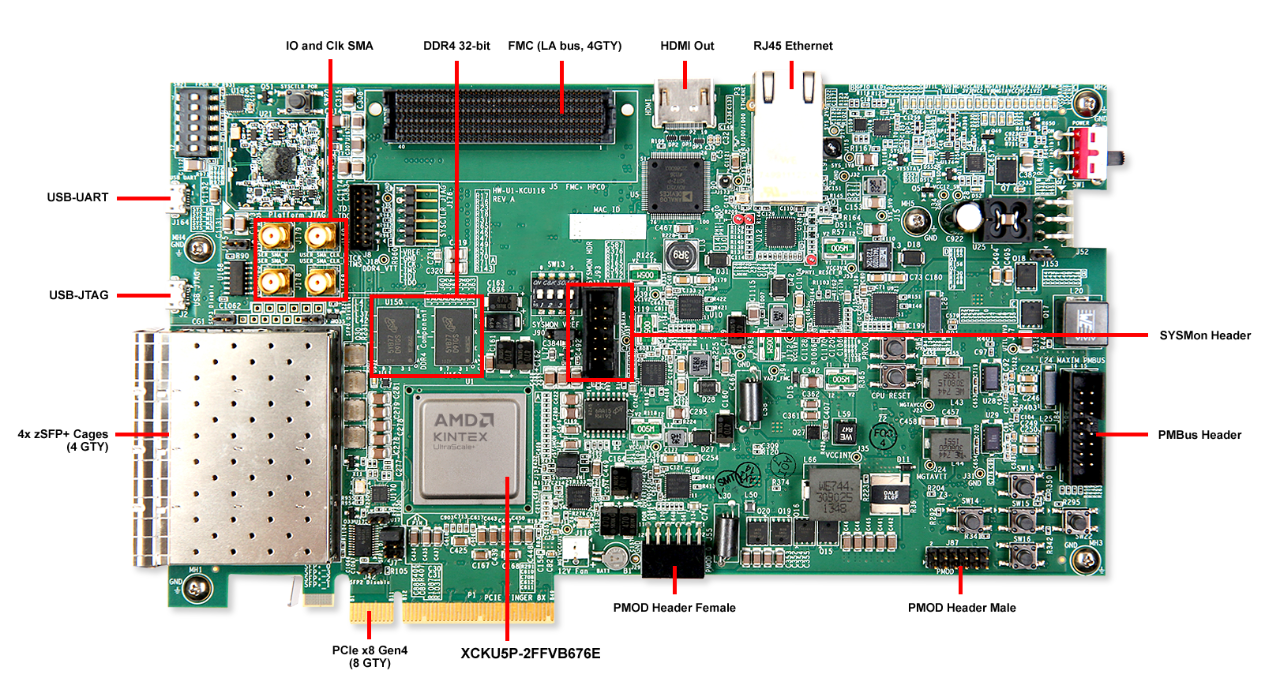
\includegraphics[width=0.7\linewidth]{kcu116}
	\caption[Carte de développement KCU116]{Carte de développement KCU116. Source : xilinx.com ref. URL04}
	\label{fig:kcu116}
\end{figure}

\section{Implémentation Solution PCIe}

\subsection{Architecture Logique}

Afin d'interfacer avec le \gls{pcie} dans le \gls{fpga}, Vivado nous met à disposition un \gls{ip} block dénommé le XDMA qui me permet d'interfacer avec celui-ci à l'aide d'un bus AXI4.

Comme pour la première solution, il me fallait mettre en place un module intermédiaire faisant le pont entre le bcrypt cracker et le XDMA.
Ce module AXI4 Attack Ctrl va contenir une \gls{bram} qui va s'occuper de stocker tous les mots de passe reçu de la part du \gls{pc}, ainsi que des registres qui vont permettre d'interagir avec le bcrypt cracker.

\begin{figure}[tbph!]
	\centering
	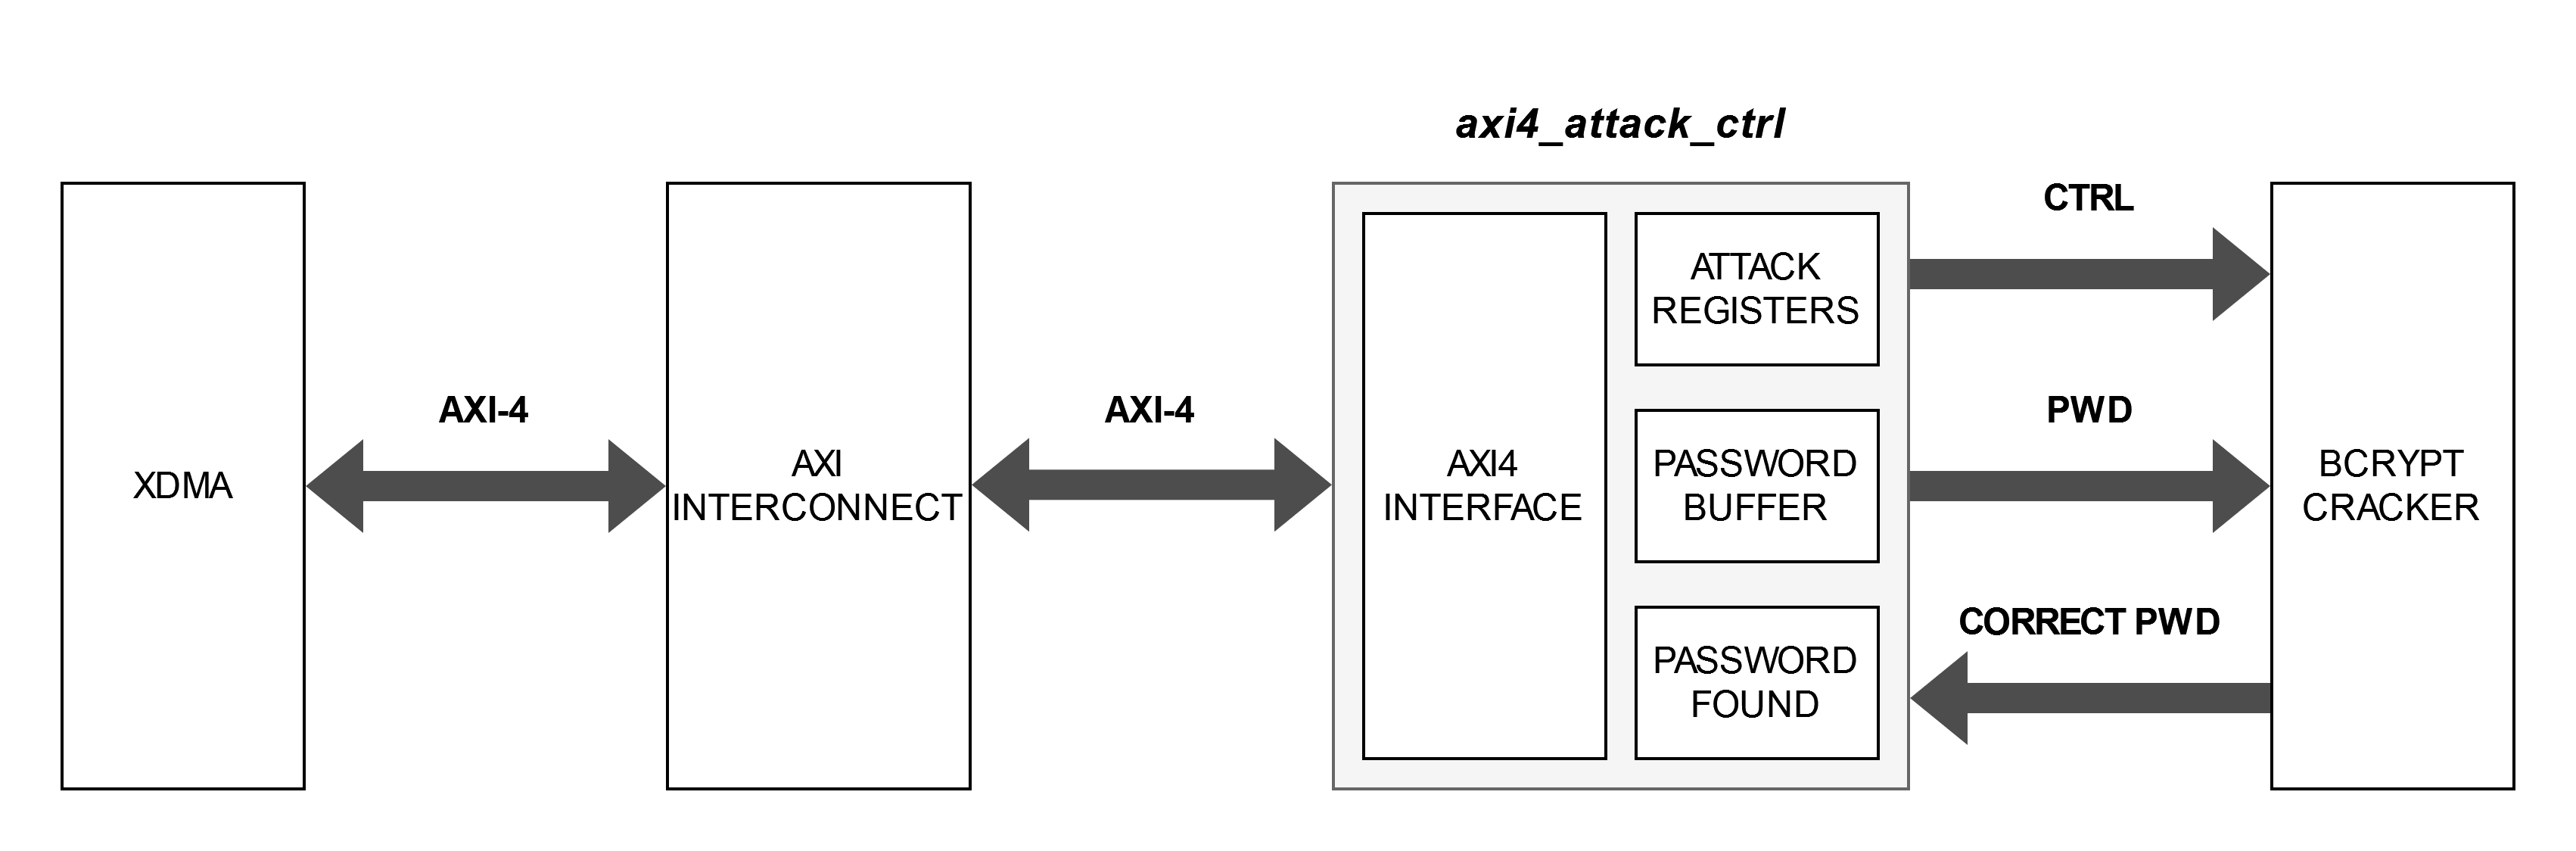
\includegraphics[width=0.8\linewidth]{pcie_top}
	\caption[Schéma Système PCIe - FPGA]{Schéma Système PCIe - FPGA. Source : réalisé par Kandiah Abivarman}
	\label{fig:pcie_top}
\end{figure}

\subsection{Implémentation sur FPGA}

J'ai très vite rencontré un problème avec l'implémentation, en effet une \gls{bram} ne peut avoir que deux ports d'accès mémoire.
Le soucis est que j'ai besoin des deux ports afin de transférer le plus rapidement possible tout le mot de passe à la \gls{bram} et j'en ai aussi besoin pour transférer les mots de passe au bcrypt cracker. 
J'ai donc mis en place un module dénommé Cracker Regs qui doit s'occuper de multiplexer l'accès mémoire entre le bcrypt cracker et le XDMA et qui s'occupe du système de registre pour le contrôle du bcrypt cracker.
J'ai aussi utilisé un \gls{ip} block me permettant d'interfacer la \gls{bram} avec de l'AXI4 ce qui va servir pour l'accès provenant de l'XDMA.

\begin{figure}[tbph!]
	\centering
	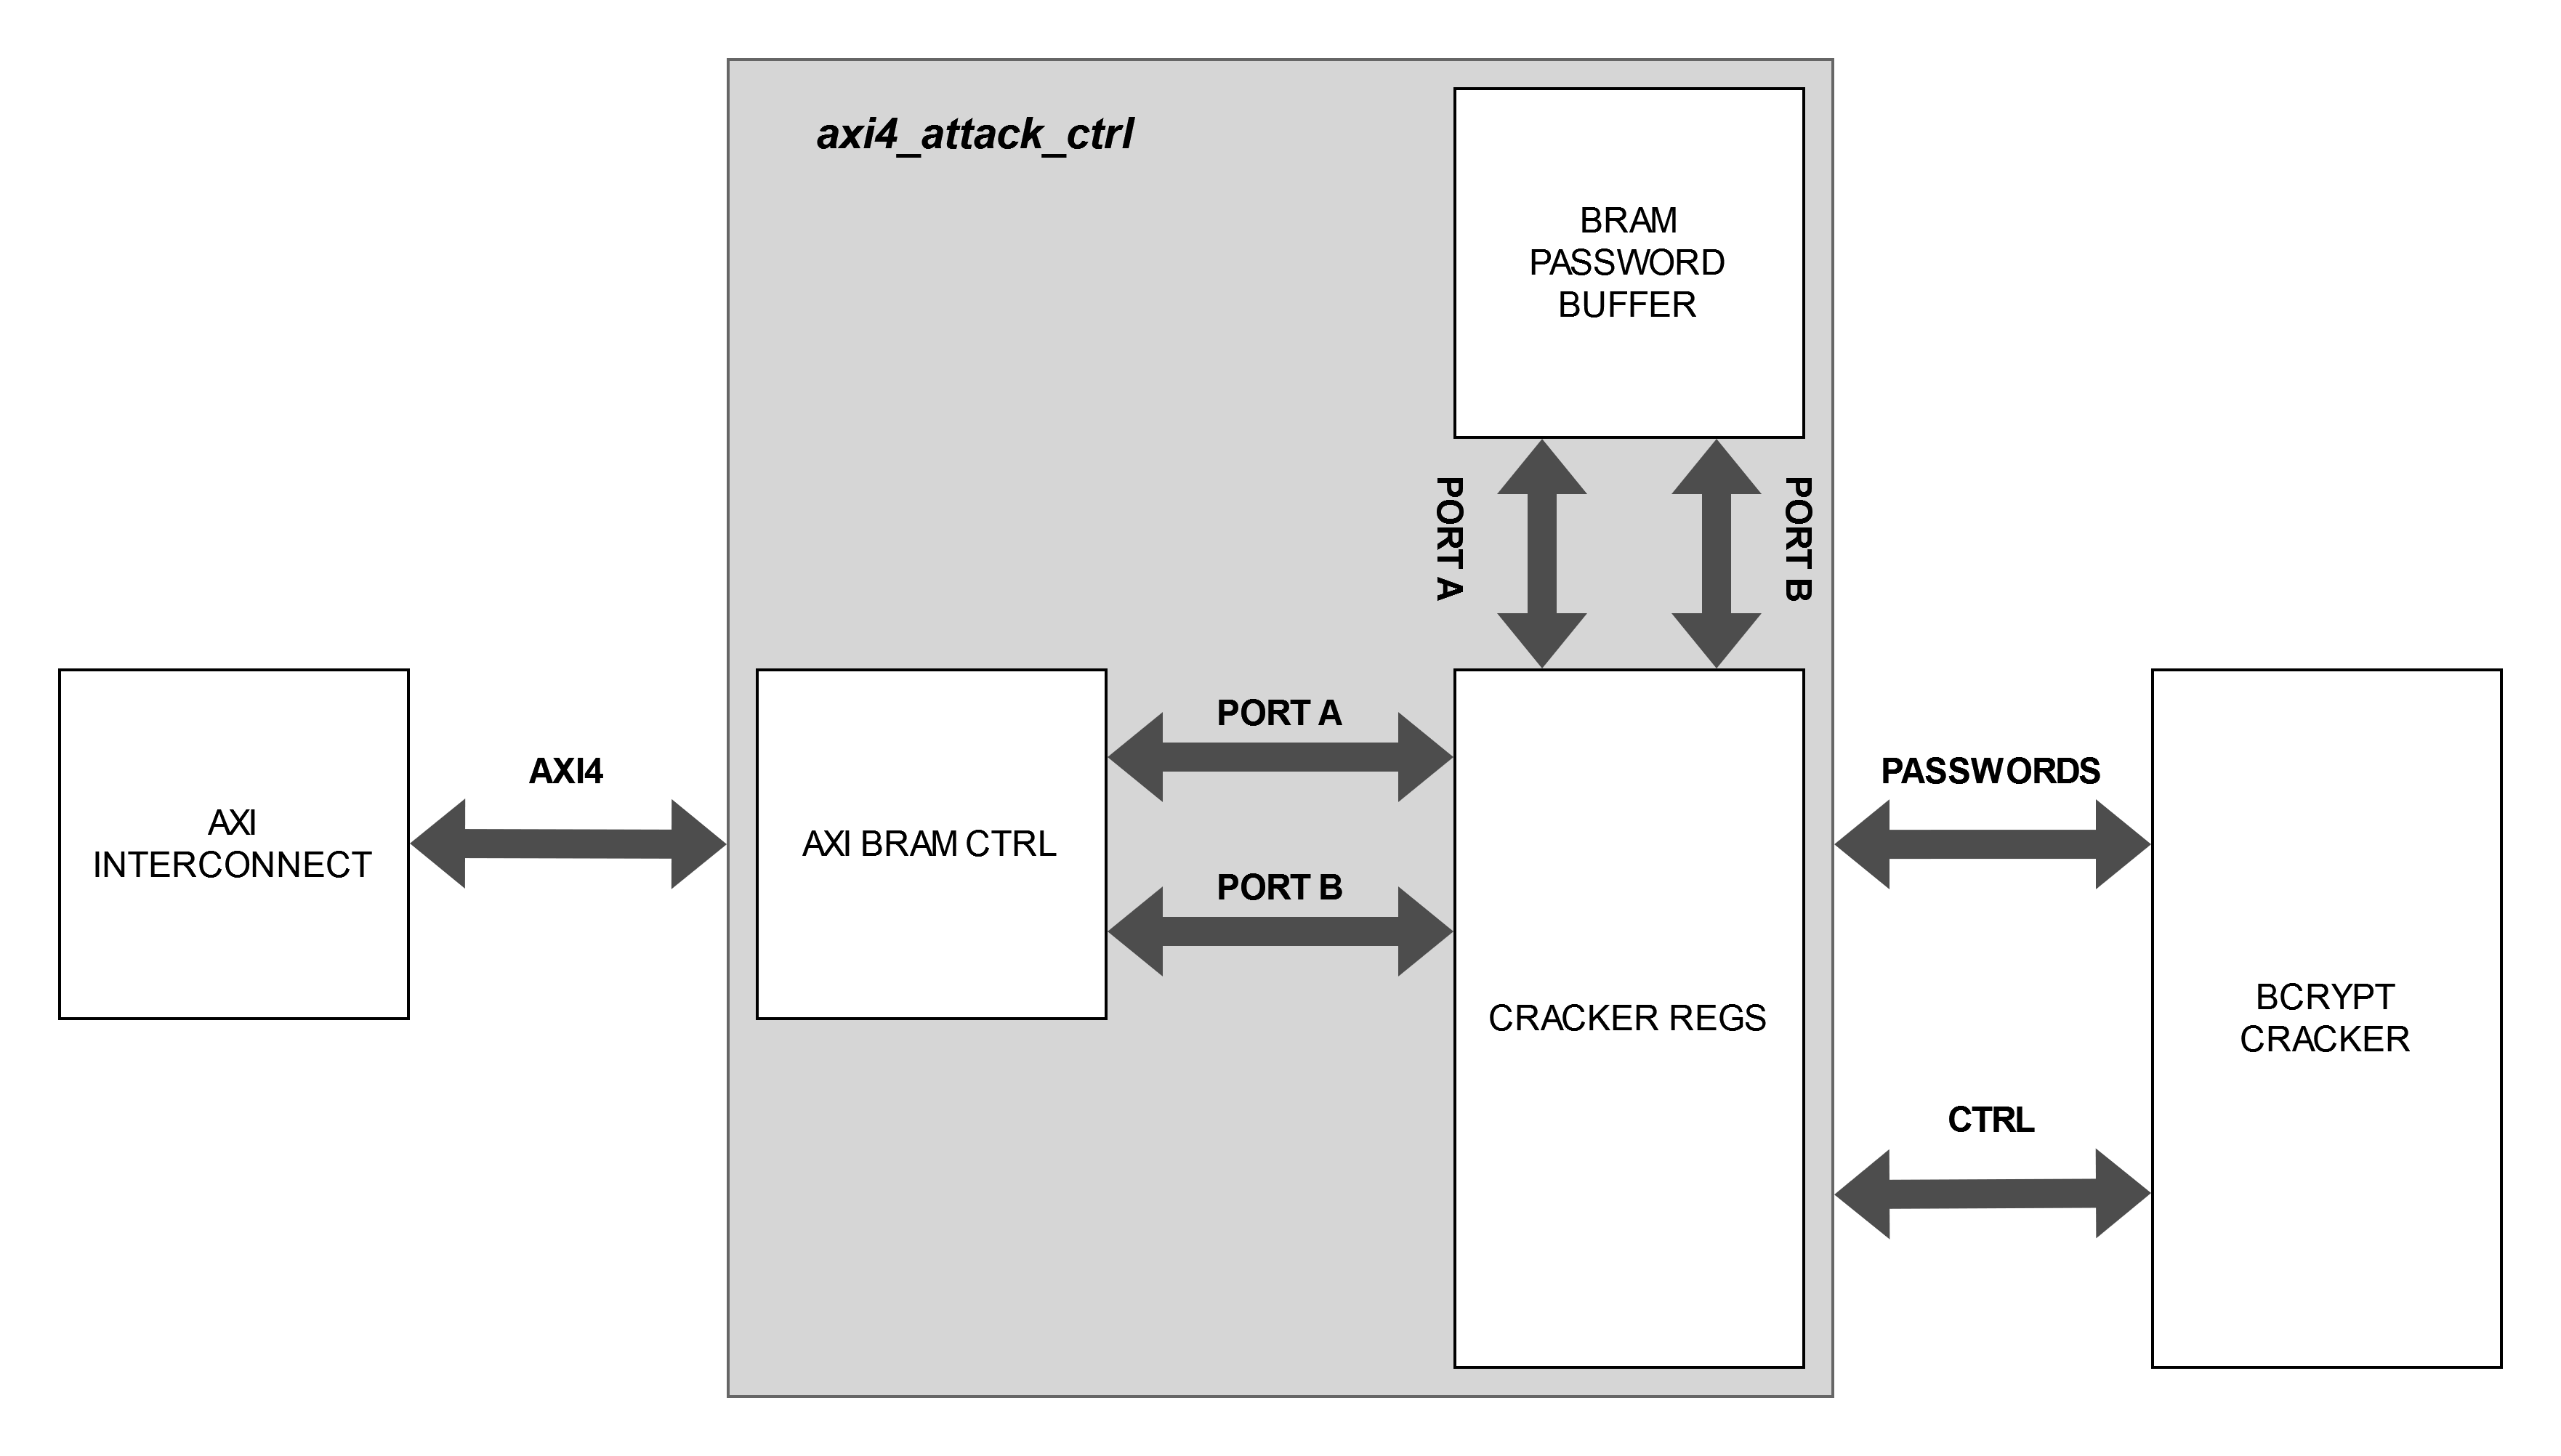
\includegraphics[width=0.8\linewidth]{pcie_axi4_attack_ctrl}
	\caption[Schéma logique AXI4 Attack Ctrl - FPGA]{Schéma logique AXI4 Attack Ctrl - FPGA. Source : réalisé par Kandiah Abivarman}
	\label{fig:pcie_axi4_attack_ctrl}
\end{figure}

\subsubsection{Implémentation Cracker Regs}

Le module Cracker Regs doit s'occuper de donner l'accès mémoire soit au \gls{pc}, soit au bcrypt cracker en fonction de l'état actuel du système.

Initialement le \gls{pc} aura la main sur la \gls{bram}, alors l'utilisateur pourra envoyer le hash et le salt que l'on souhaite casser et tous les mots de passe nécessaire au bcrypt quadcore présents.
Puis lorsque l'on aura écrit sur le registre start, le bcrypt cracker prendra la main sur la \gls{bram} le temps de distribuer tous les mots de passe au différents quadcore.
l'ordinateur n'aura pas le droit d'écrire dans la mémoire et lors d'une lecture, il recevra la valeur actuelle dans le registre start. 
Lorsque le bcrypt cracker aura fini de récupérer tous les mots de passe, le registre start repassera à zéro et le module Cracker Regs redonnera la main à l'ordinateur pour qu'il puisse envoyer les prochains mots de passe.

Les mots de passe, le hash, le salt et le registre d'attaque sont tous stockés à des adresses spécifiques, les adresses vont dépendre du nombre de quadcores.

\begin{figure}[tbph!]
	\centering
	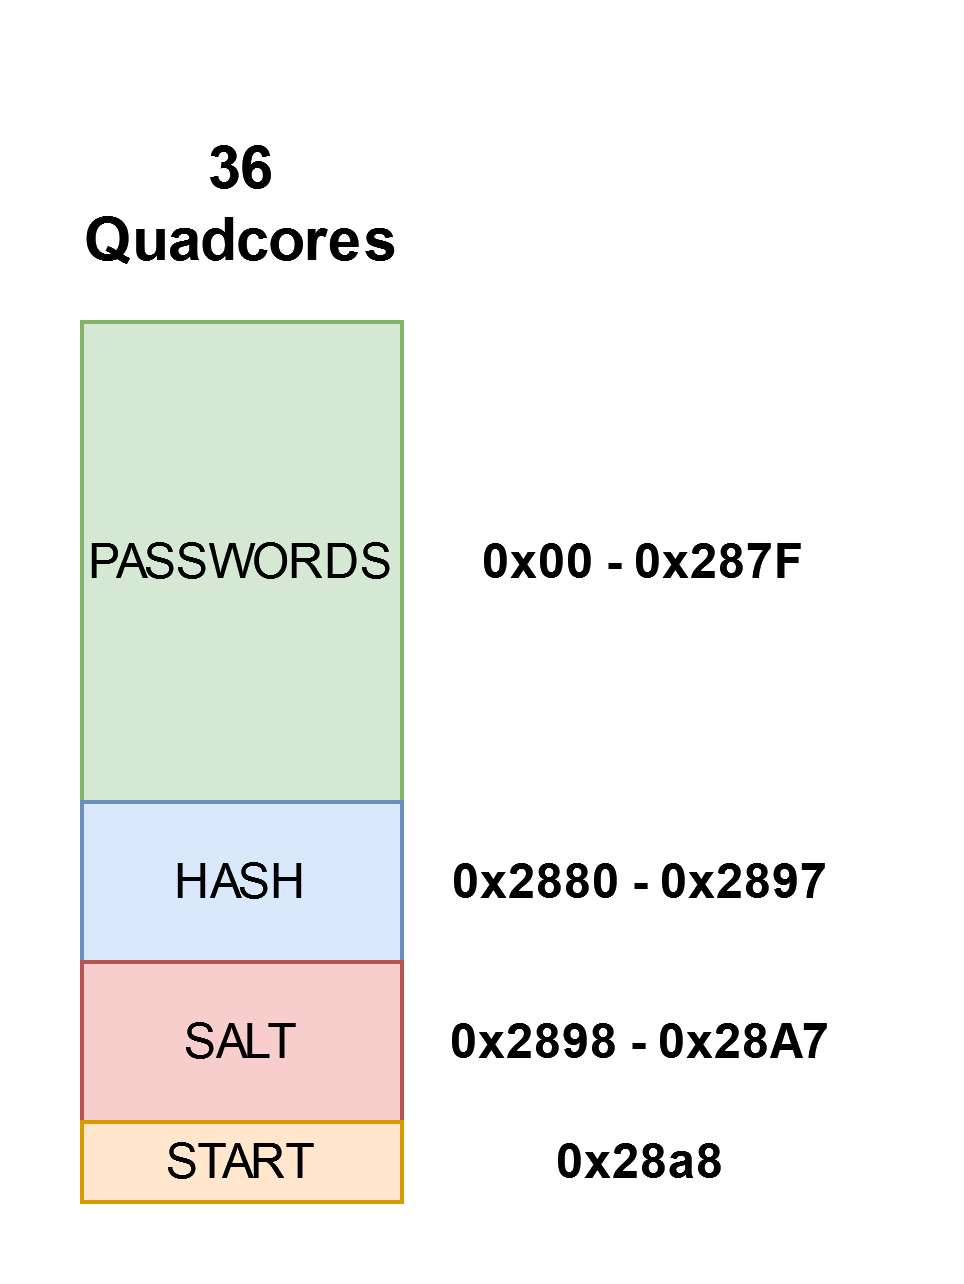
\includegraphics[width=0.4\linewidth]{pcie_bram_addresses}
	\caption[BRAM Adresses - FPGA]{BRAM Adresses - FPGA. Source : réalisé par Kandiah Abivarman}
	\label{fig:pcie_bram_addresses}
\end{figure}

\subsubsection{Modifications Bcrypt Cracker}

J'ai tout d'abord modifié le bcrypt quadcore en enlevant le générateur de mots de passe.
Puis comme pour la première solution, j'ai ajouté deux états supplémentaires d'attente, une première qui va attendre de recevoir les mots de passe a tester et une deuxième qui va attendre que les autres quadcores soient prêt pour l'initialisation de la mémoire.

Puis j'ai modifié le bcrypt cracker pour qu'il puisse récupérer les mots de passe et les distribuer au quadcores.
J'ai aussi fait en sorte d'avertir le Cracker Regs lorsque tous les mots de passe ont été récupérés.

\subsection{Vérification Hardware}

Afin de gagner du temps pour la vérification, j'ai décidé de remplacer le \gls{pcie} par un microblaze qui est un \gls{ip} bloc fourni par Vivado qui fait office de microcontrôleur.
Ainsi, le microblaze pourra prendre la place de l'XDMA et je pourrai mettre en place un code C afin de tester aisément le fonctionnement de mon système.
Si le système est fonctionnel de cette manière, alors normalement mon système devrait marcher aussi avec le \gls{pcie}.
Afin de vérifier si le mots de passe a bien été trouvé, j'ai mis les interfaces du bcrypt cracker sur des \gls{ip} \gls{gpio}s qui sont adressable par AXI4 afin d'éviter de trop compléxifier le module Cracker Regs.

\begin{figure}[tbph!]
	\centering
	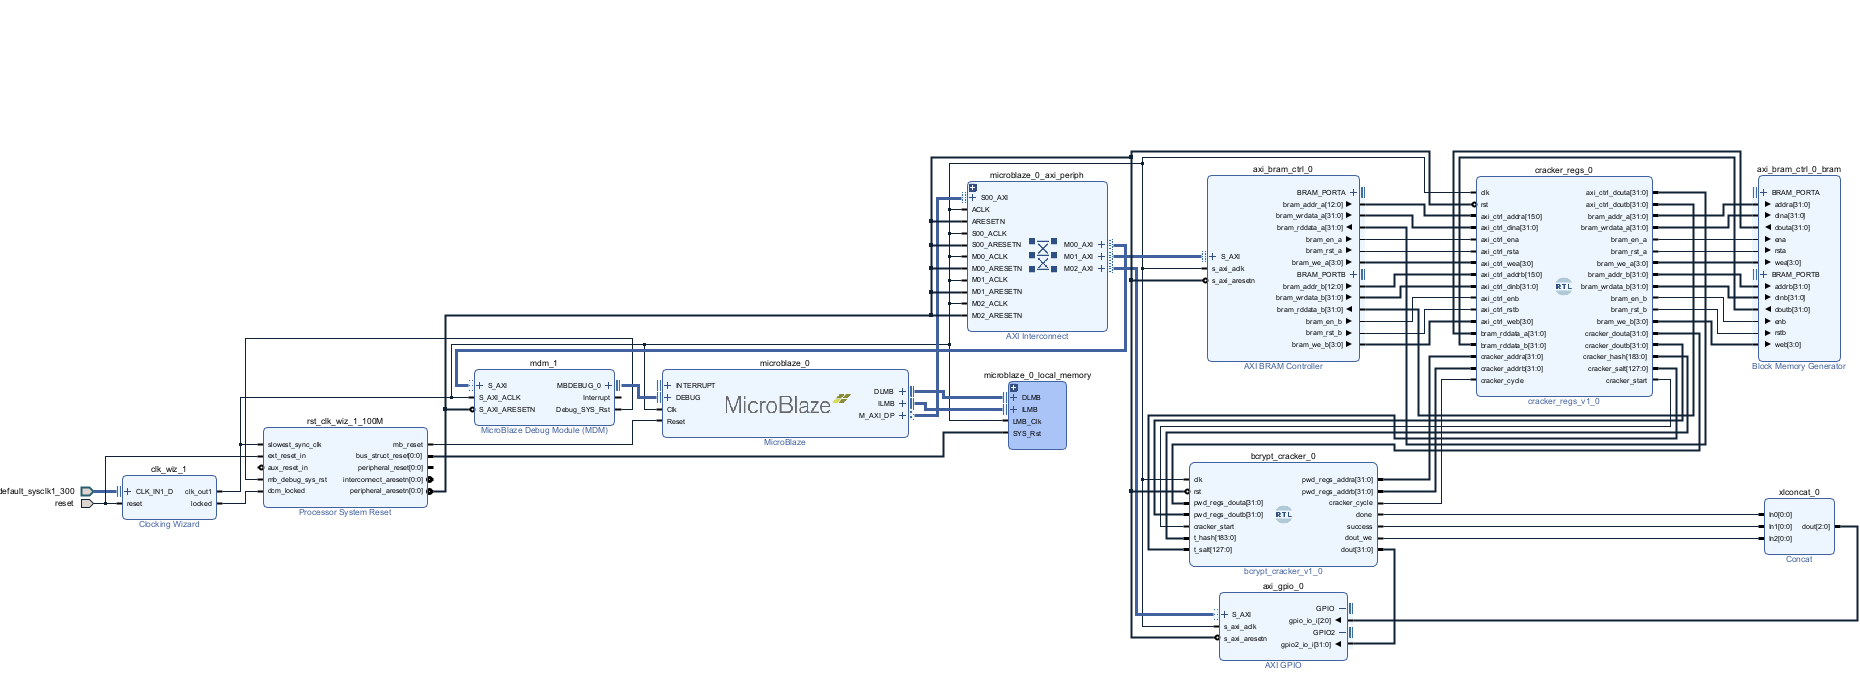
\includegraphics[width=1.4\linewidth, angle=-90]{pcie_test_db}
	\caption[Block Design Test PCIe - FPGA]{Block Design Test PCIe - FPGA. Source : réalisé par Kandiah Abivarman}
	\label{fig:pcie_test_db}
\end{figure}

Malgré de nombreuses heures passées à faire du debug, je n'ai malheureusement pas réussi à faire marcher le système.
Par manque de temps, j'ai décidé de tester directement sans passer par la simulation, en utilisant les outils de debug qui sont mis à disposition par Vivado.
J'ai pu identifier et réglé quelques problèmes, mais le système n'est toujours pas fonctionnel.